\documentclass[12pt]{article}
\usepackage{titlesec}
\usepackage{float}
\usepackage{graphicx}

\usepackage{hyperref}
\hypersetup{
    colorlinks,
    citecolor=black,
    filecolor=black,
    linkcolor=black,
    urlcolor=black
}

\begin{document}

\title{User Manual} 
\author{Team: The Outsiders\\ \\ Kirk Montour (montour)\\ Syed Gardezi (gardezsh)}
\date{\today}
  
\maketitle

\pagebreak

\tableofcontents

\pagebreak

\section{Introduction}

\subsection{Purpose}
To train a user to be able to administrate their website by doing common web administration tasks after minimal training with the assistance of this User Manual.

\subsection{Scope}
The scope of the user manual is to provide step by step instructions to execute the ''common cases'' pertaining to web administration and to lay a solid foundation for learning intuitively.

\subsection{Background}
Our Content Management System is a web application for non-technical users to manage and maintain their own website, which reduces web maintenance costs. Our User Manual will be very clear and concise, and should need to be consulted only a few times for mastery of web administration common cases.

\subsection{Roadmap}

\begin{enumerate}
  \item User instructions for logging into the administration site, through the login system
  \item User instructions for common User Management tasks
  \item User instructions for common Page Management tasks
  \item User instructions for setting the theme of the website
\end{enumerate}

\section{Tasks}

\subsection{Logging into the administration area}

\begin{enumerate}
  \item Enter the URL of the Administration site into the address bar of the browser. The URL of the Administration site is the name of the site plus the cap.admin directory appended to the name of the site. In this instance, the site is http://localhost/ for an http://localhost/cap.admin administration site. Navigate to the Administration site login page by entering the Administration site URL and pressing enter.
  
  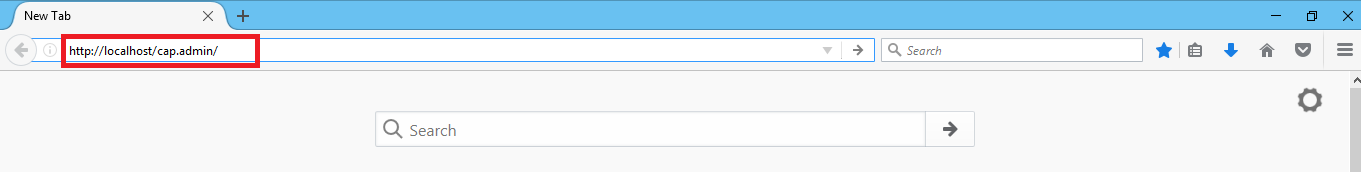
\includegraphics[width=\textwidth,height=\textheight,keepaspectratio]{pics/login.png}
  
  \item This takes you to the Administration site login page.
  
  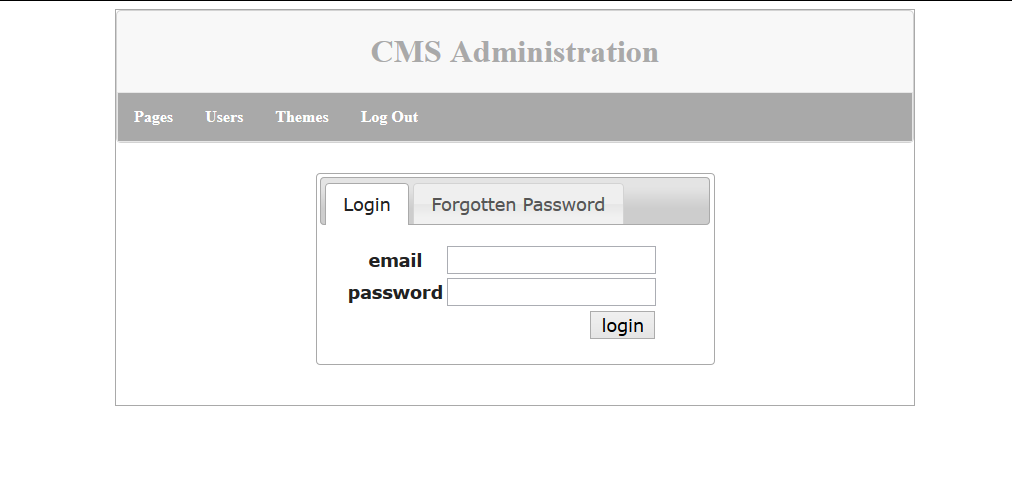
\includegraphics[width=\textwidth,height=\textheight,keepaspectratio]{pics/adminLoginPage.png}
  
  
  \item On the Administration site login page, type in a valid user email and password into the email input box and the password input box, and press enter.
  
  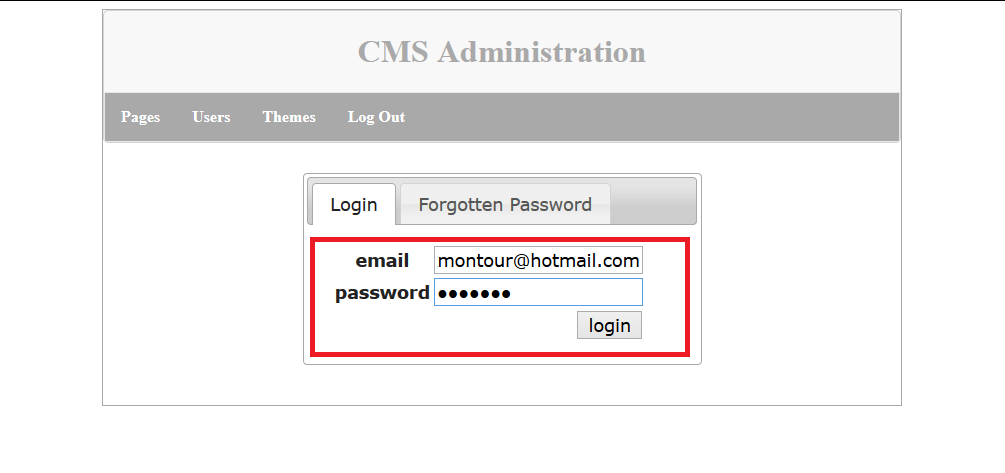
\includegraphics[width=\textwidth,height=\textheight,keepaspectratio]{pics/emailPassword.png}
  
  \item This action will take us to the CMS Administration site, which by default takes us to the Page Management Administration page, and we are successfully logged into the CMS Administration site.
  
  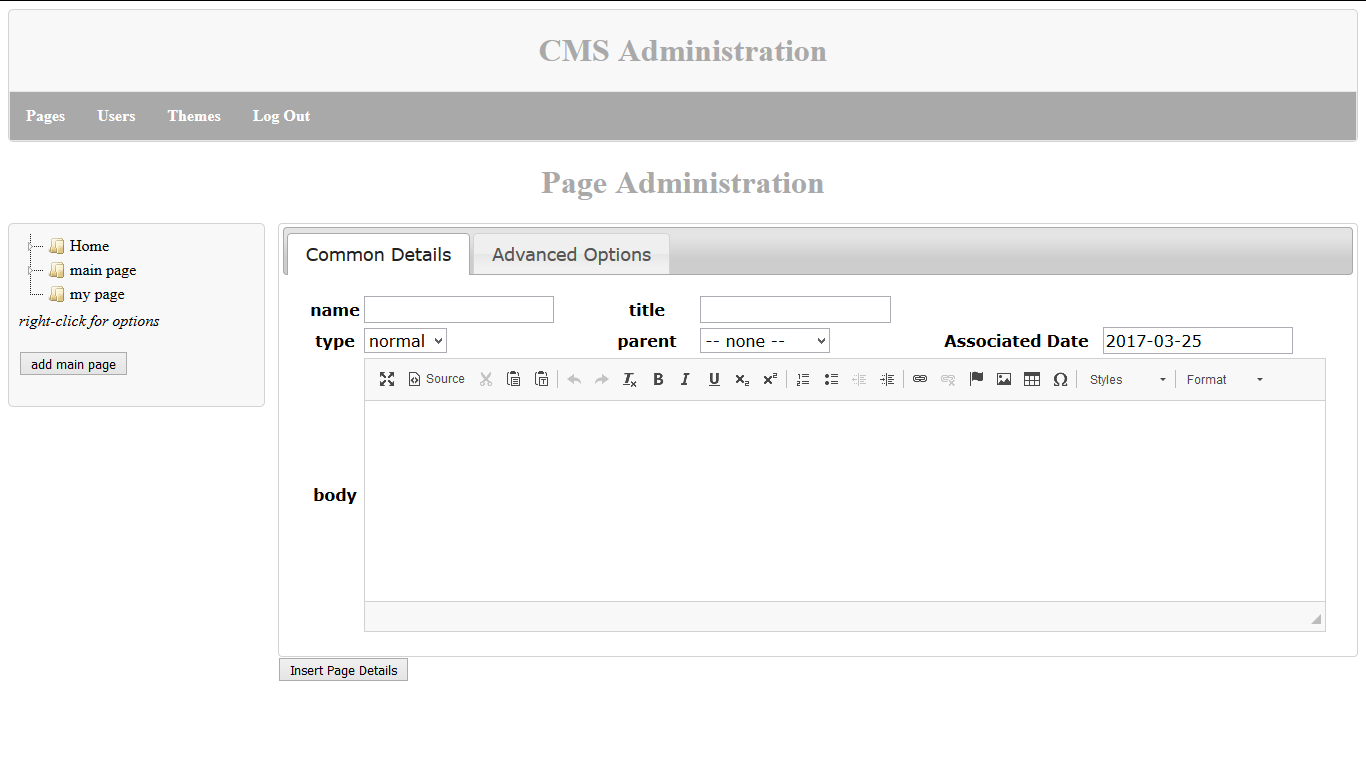
\includegraphics[width=\textwidth,height=\textheight,keepaspectratio]{pics/pageAdmin.png}

\end{enumerate}

\subsection{Create basic user}

\begin{enumerate}
  \item Login to the administration web site (see above Login instructions). This brings you by default to the Page Management system.
  
  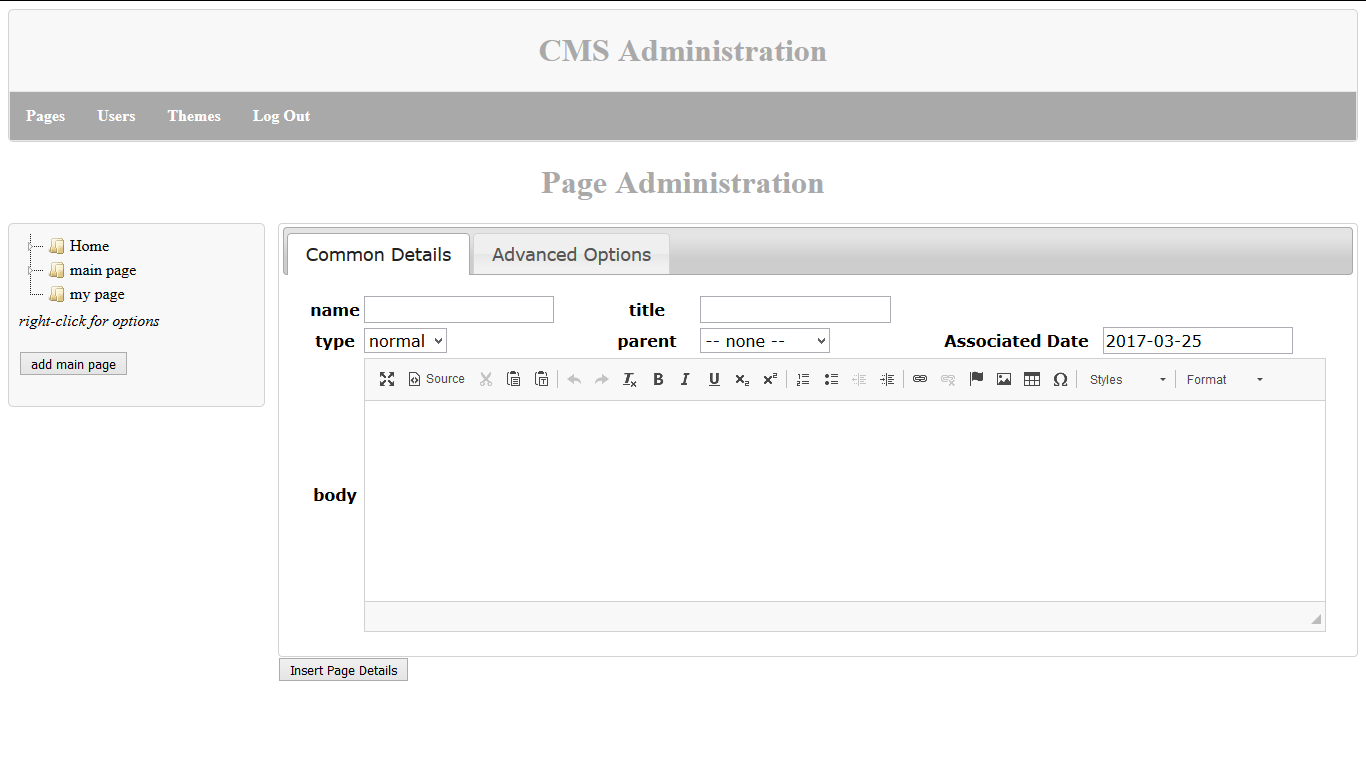
\includegraphics[width=\textwidth,height=\textheight,keepaspectratio]{pics/createBasicUser_1.png}
  
  \item Click the Users link in the CMS Administration menu.
  
  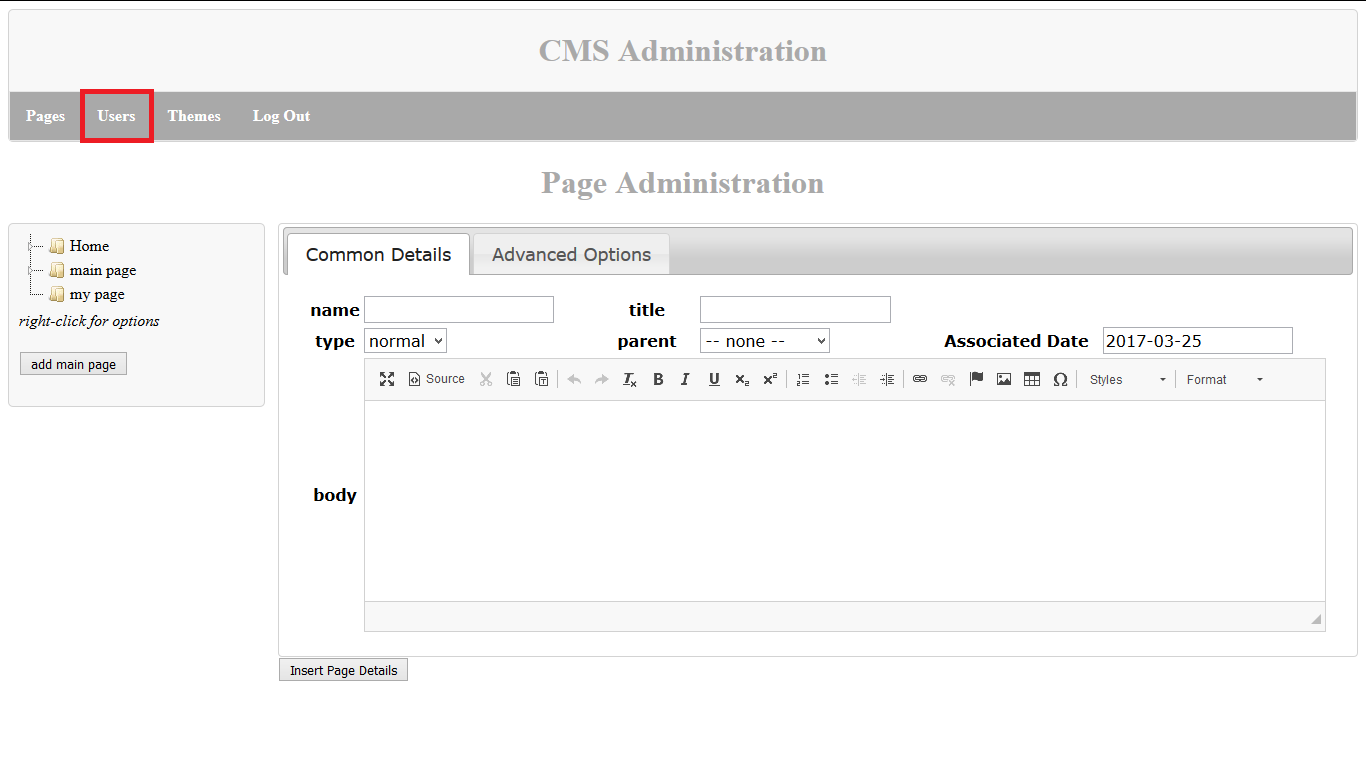
\includegraphics[width=\textwidth,height=\textheight,keepaspectratio]{pics/createBasicUser_2.png}
  
  \pagebreak
  
  \item This takes you to the User Management Page.
  
  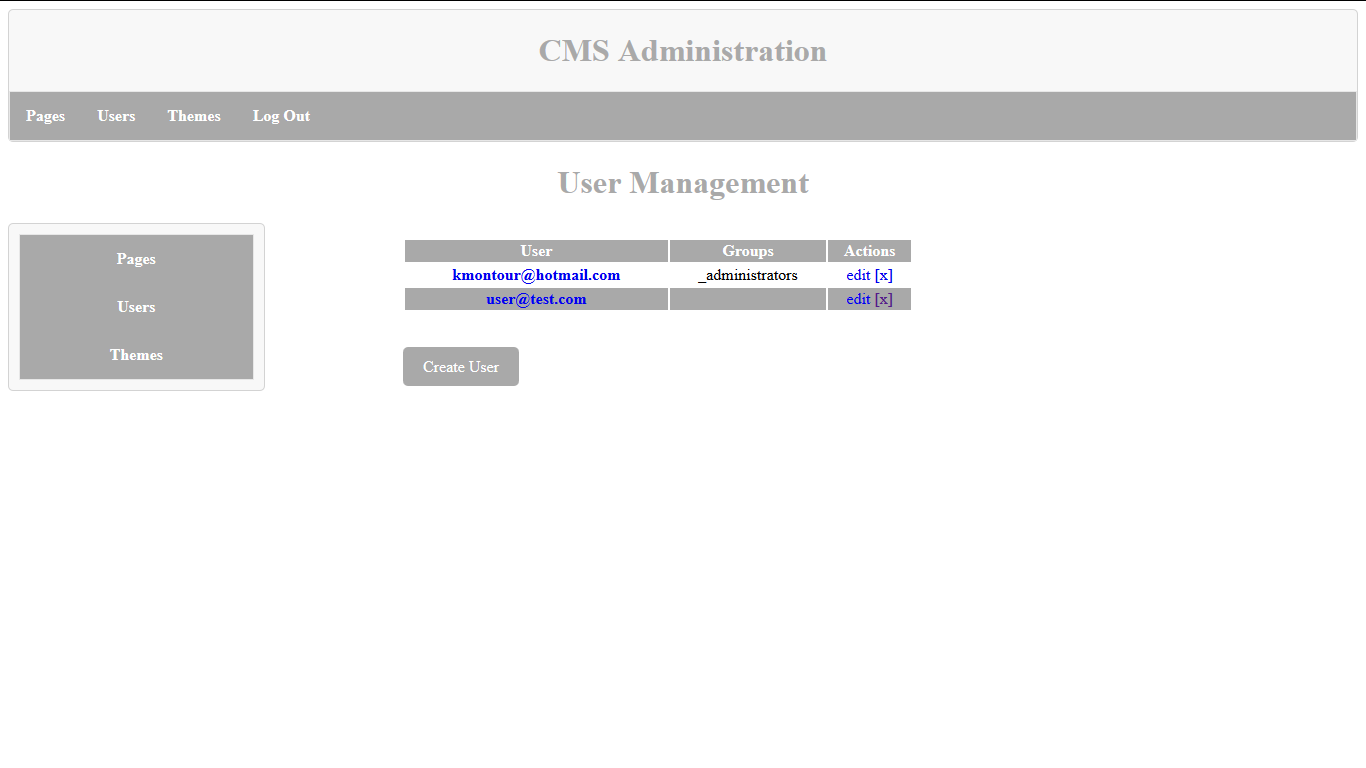
\includegraphics[width=\textwidth,height=\textheight,keepaspectratio]{pics/createBasicUser_3.png}
  
  \item Click the ''Create User'' button.
  
  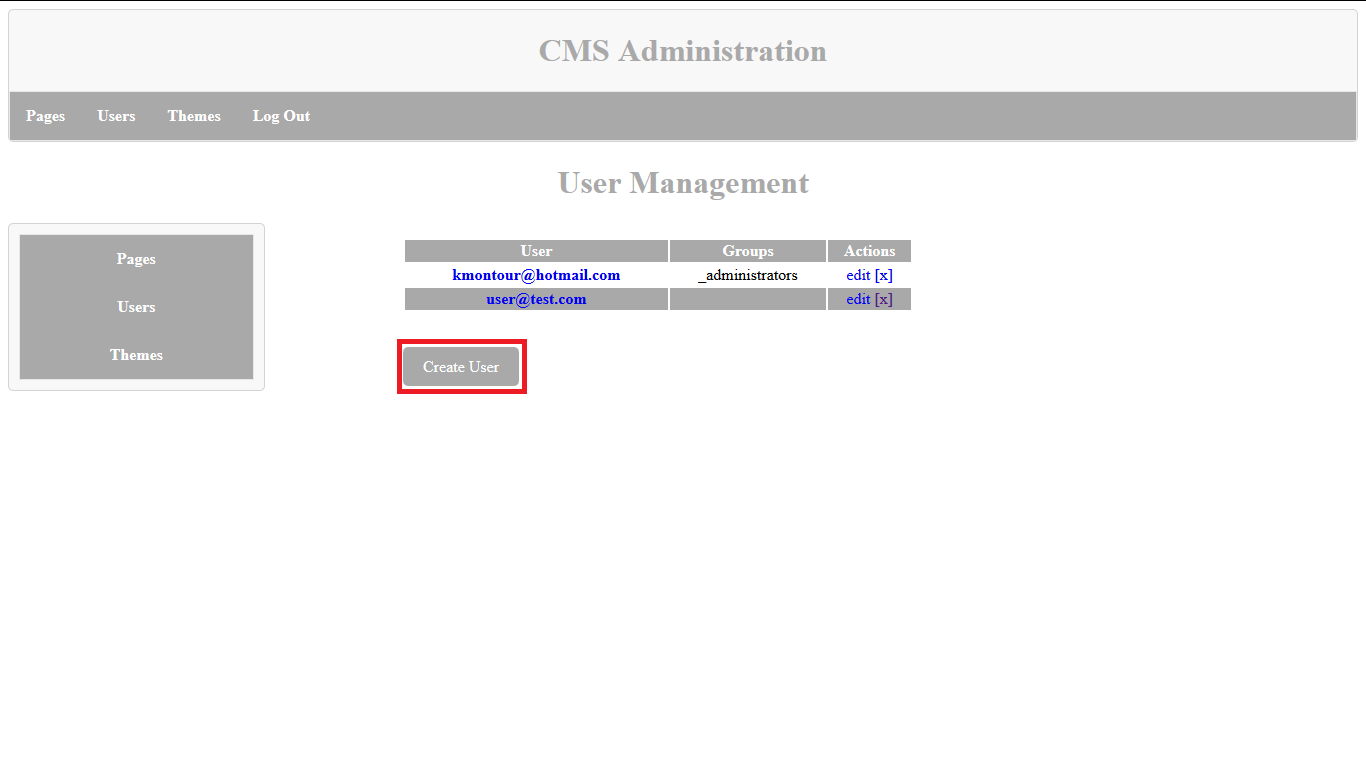
\includegraphics[width=\textwidth,height=\textheight,keepaspectratio]{pics/createBasicUser_4.png}
  
  \pagebreak
  
  \item Clicking the ''Create User'' button reveals a form for creating new users.
  
  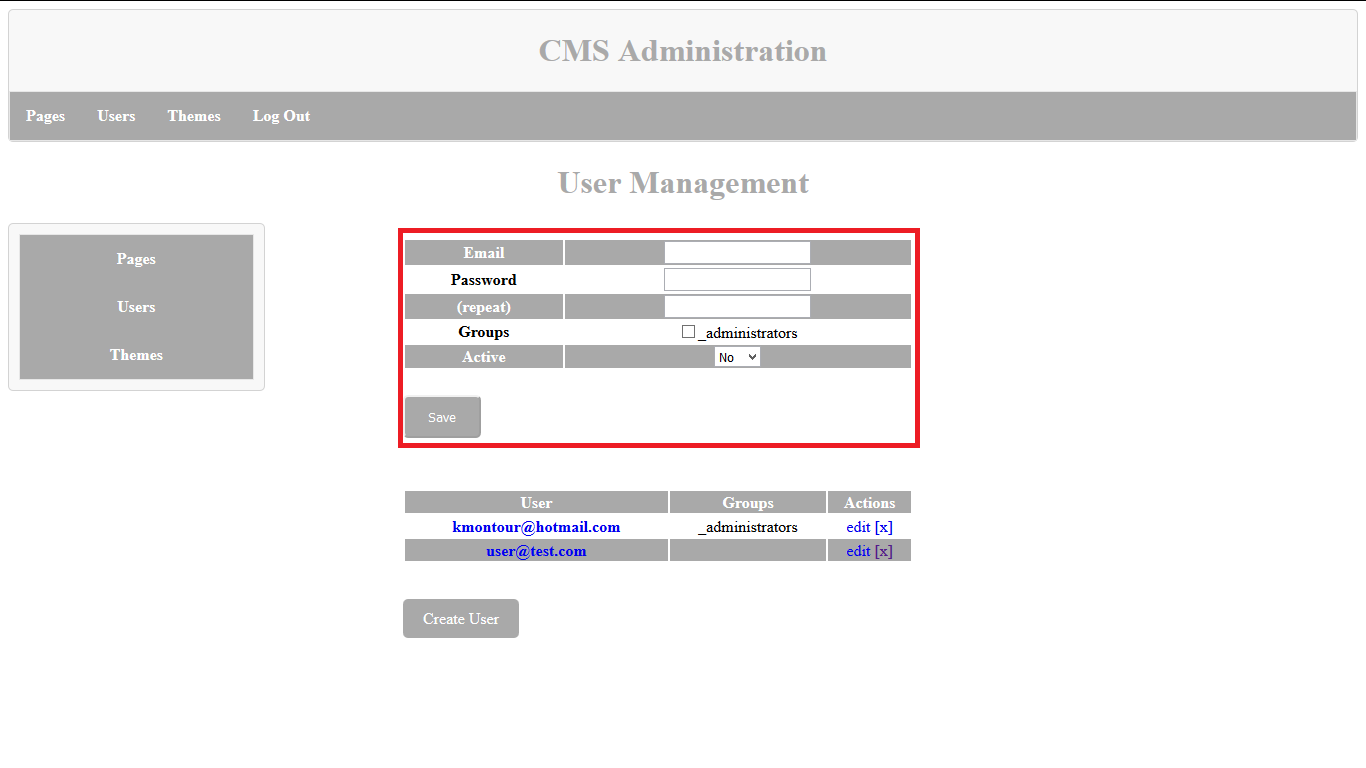
\includegraphics[width=\textwidth,height=\textheight,keepaspectratio]{pics/createBasicUser_5.png}
  
  \item Enter an email address and password into the Email input box, Password input box, and Password Confirmation input box, and click the ''Save'' button.
  
  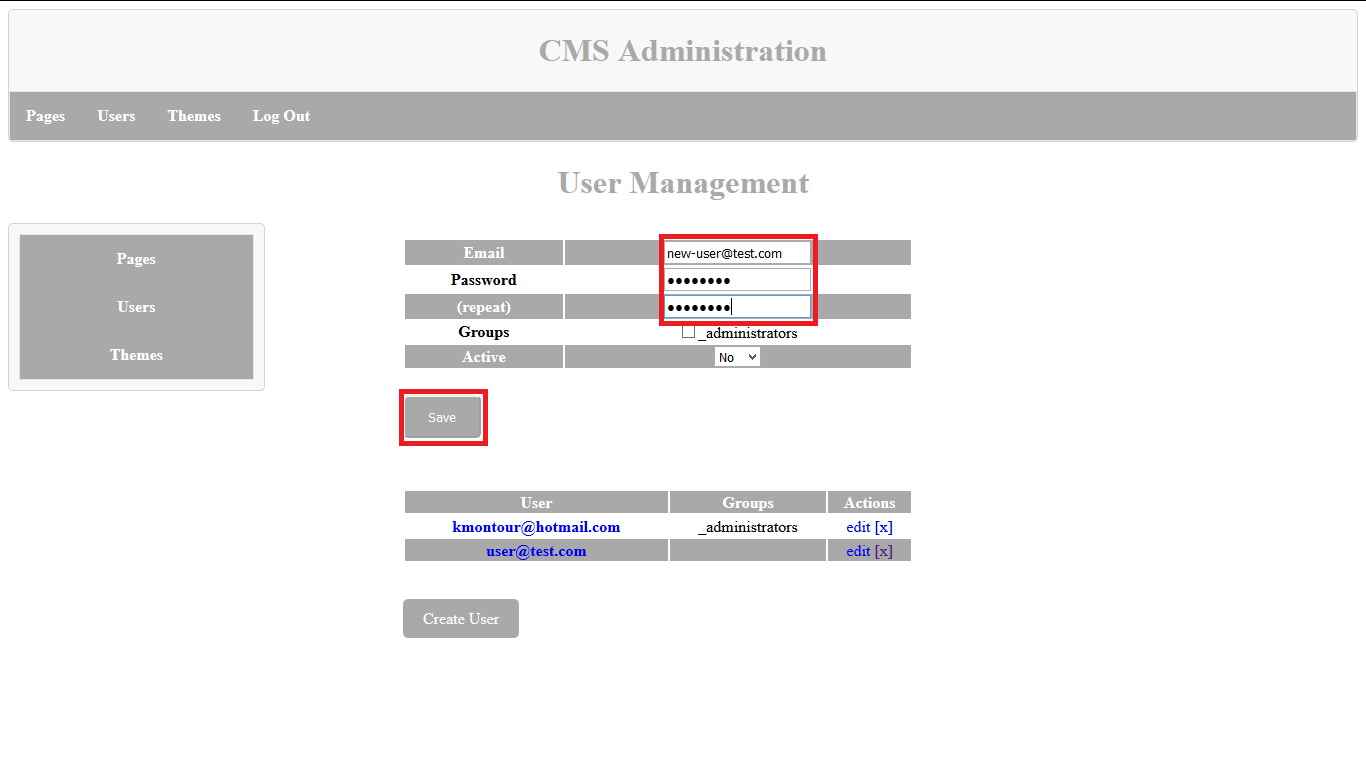
\includegraphics[width=\textwidth,height=\textheight,keepaspectratio]{pics/createBasicUser_6.png}
  
  \pagebreak
  
  \item The newly created user now shows up in the list of user accounts.
  
  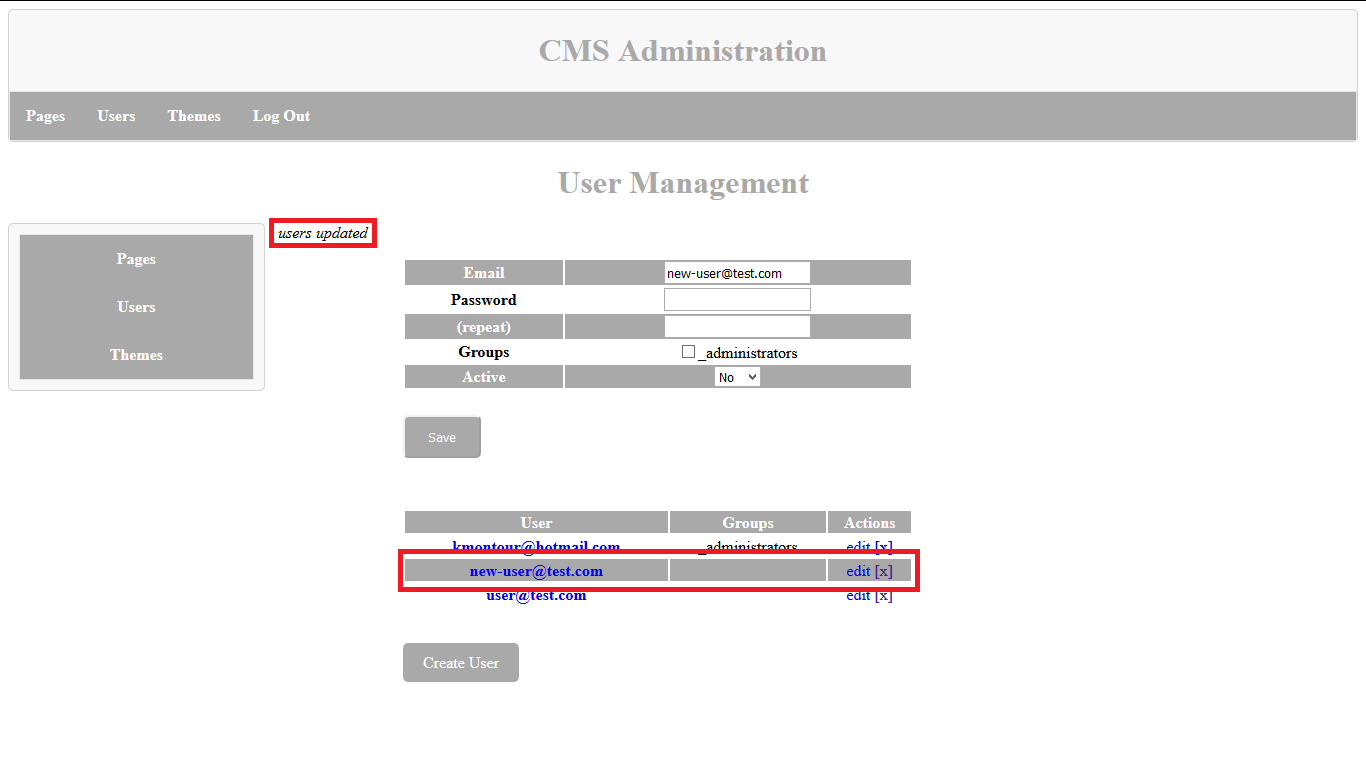
\includegraphics[width=\textwidth,height=\textheight,keepaspectratio]{pics/createBasicUser_7.png}
  
\end{enumerate}


\subsection{Edit User}

\begin{enumerate}
  \item To edit user accounts, navigate to the User Management page (see instructions for creating a basic user). This brings you to the User Management page.
  
  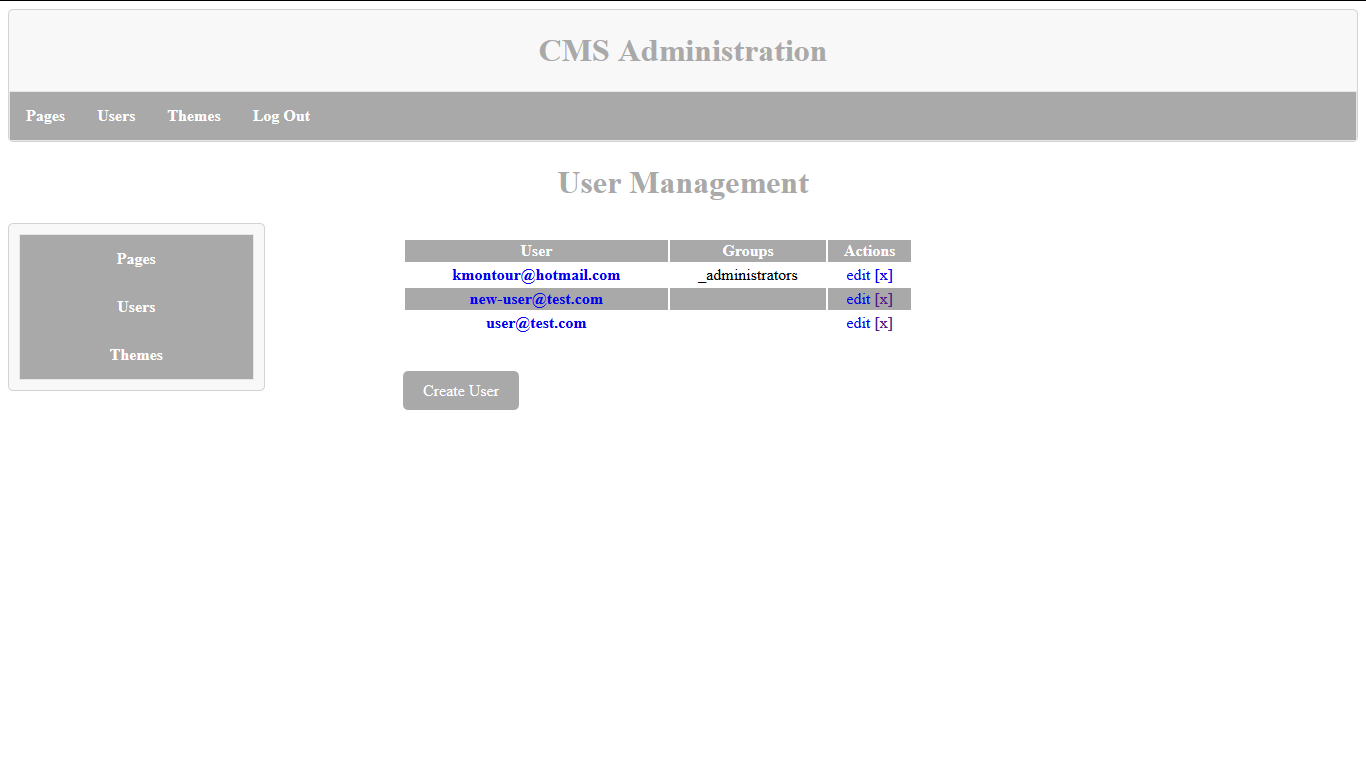
\includegraphics[width=\textwidth,height=\textheight,keepaspectratio]{pics/editUser_1.png}
  
  
  \item To edit a user account, click the edit link pertaining to the user account that you want to edit.
  
  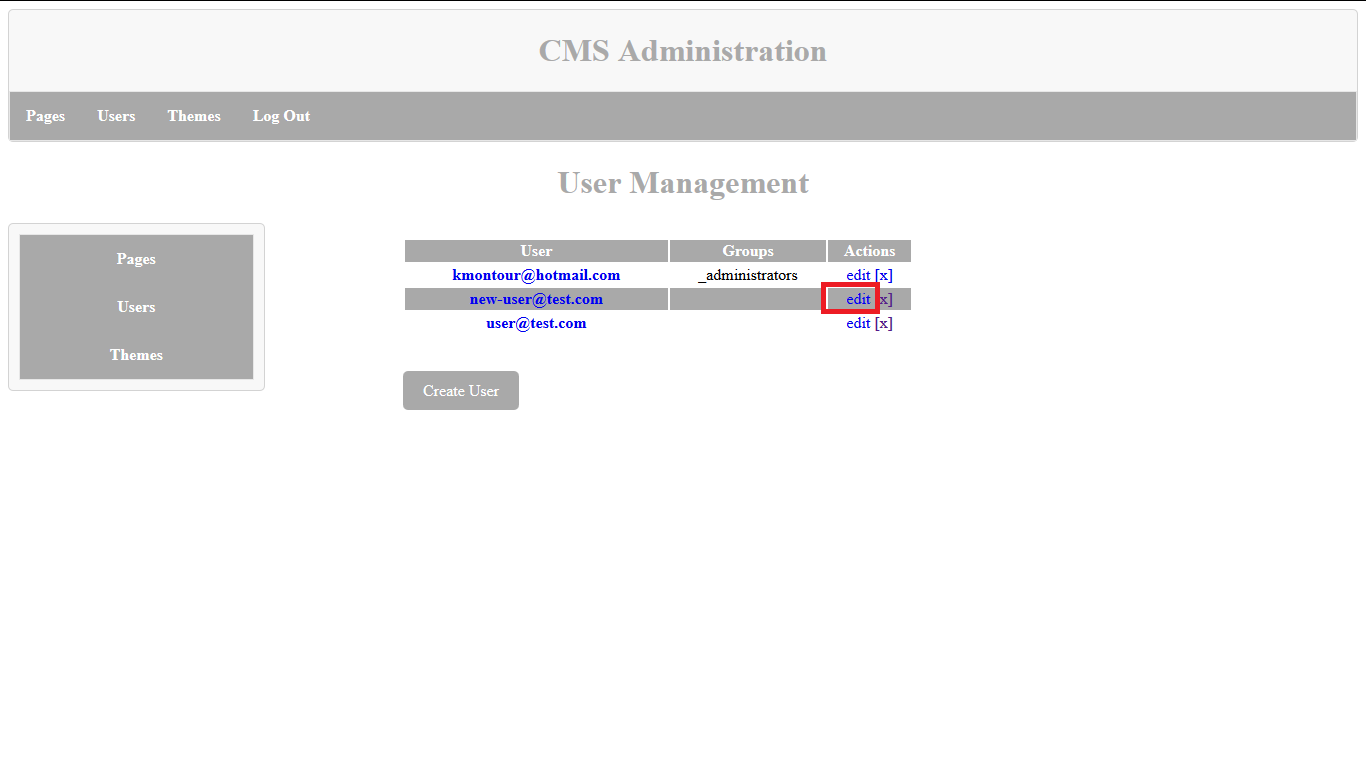
\includegraphics[width=\textwidth,height=\textheight,keepaspectratio]{pics/editUser_2.png}
  
  \item Clicking the edit link for a user account brings up a form for editing the selected user account.
  
  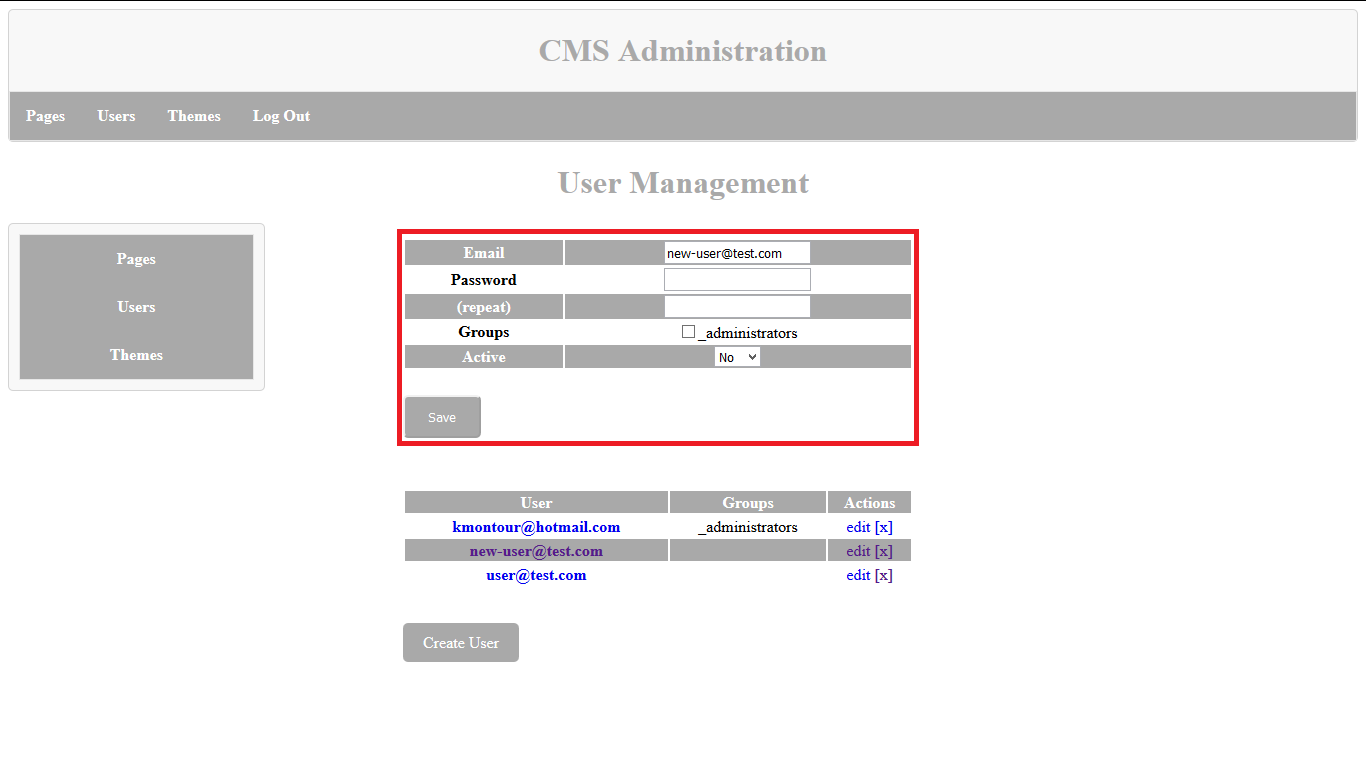
\includegraphics[width=\textwidth,height=\textheight,keepaspectratio]{pics/editUser_3.png}
  
  \item Once the user account data has been loaded into the form, it can be edited. In this example, we will add a user to the administrators group, and make the account active. Once these two options have been selected, click the ''Save'' button.  
  
  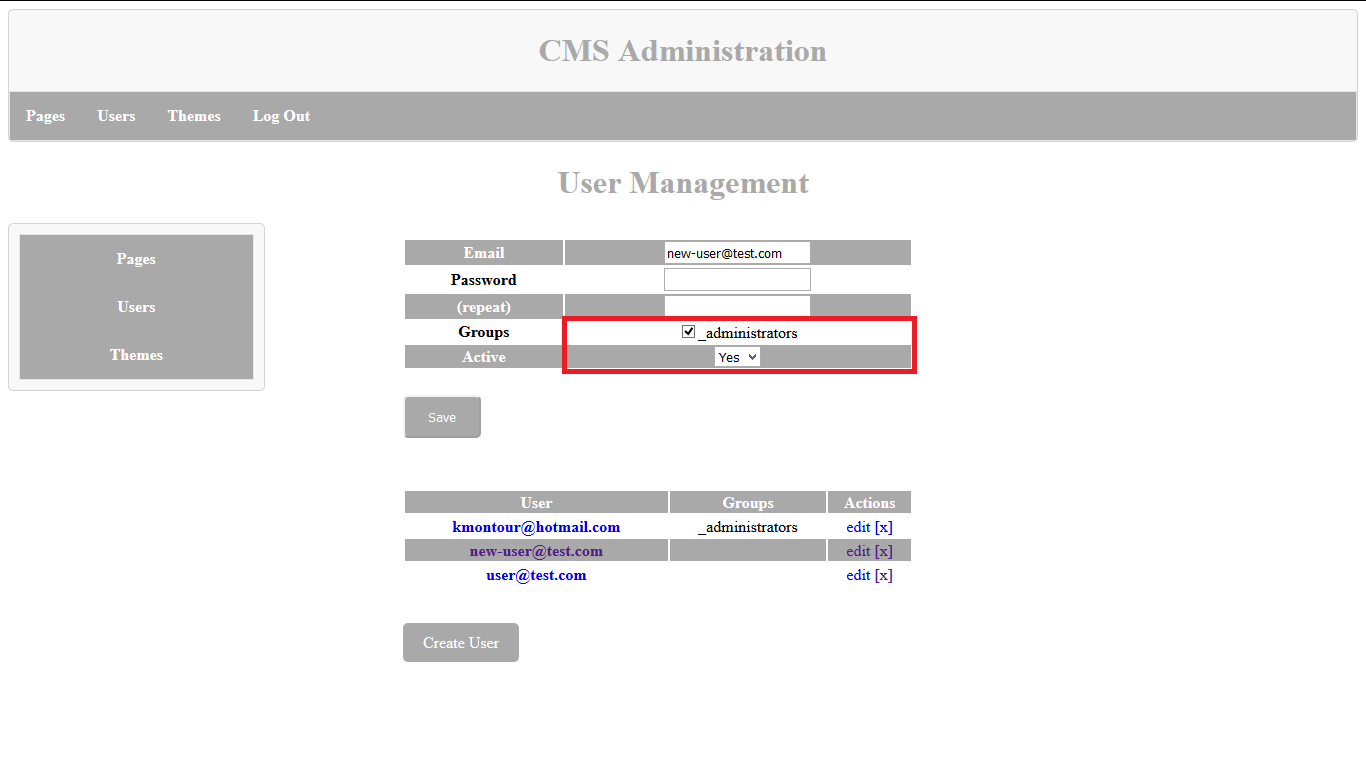
\includegraphics[width=\textwidth,height=\textheight,keepaspectratio]{pics/editUser_4.png}
  
  \item The user account data will be updated, and the new selections will be reflected in the user account list, and the edit user form.
  
  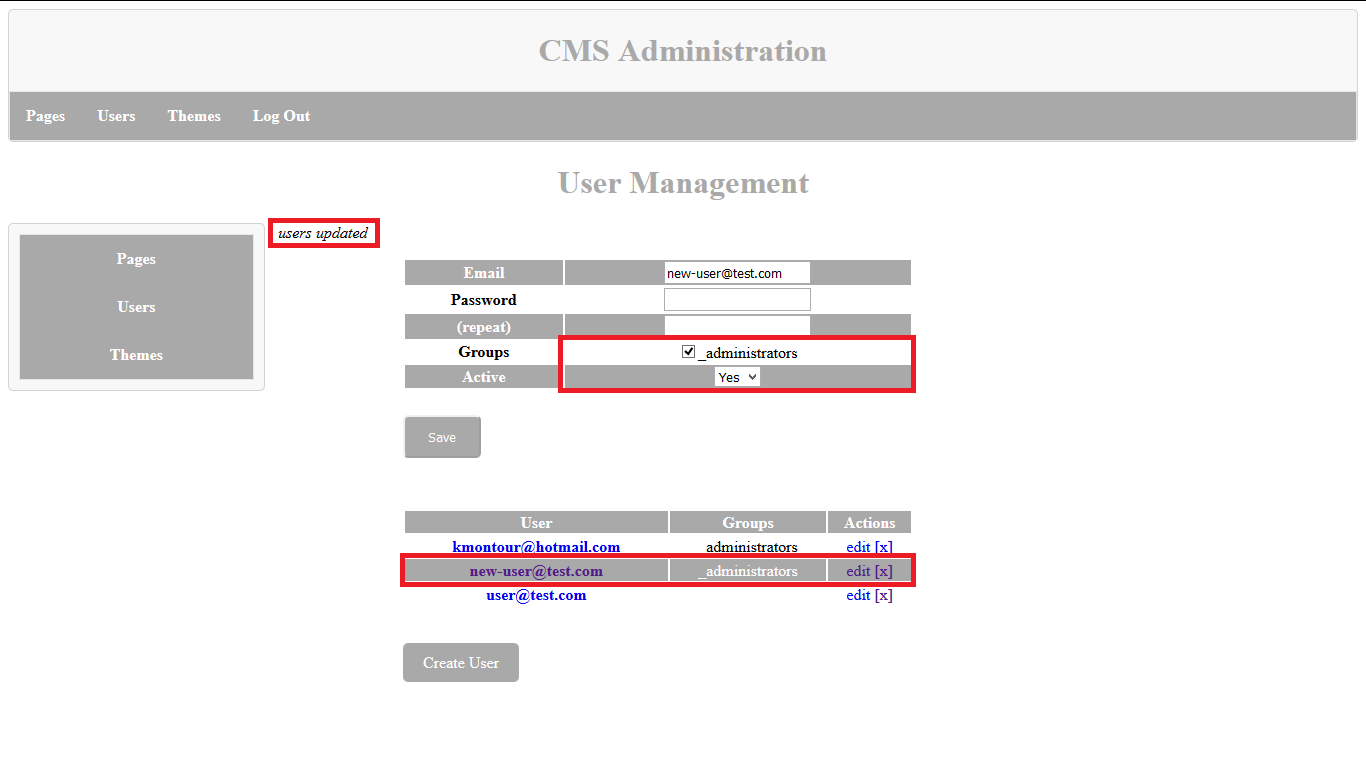
\includegraphics[width=\textwidth,height=\textheight,keepaspectratio]{pics/editUser_5.png}

\end{enumerate}

\subsection{Delete User}

\begin{enumerate}
  \item To delete user accounts, navigate to the User Management page (see instructions for creating a basic user). This brings you to the User Management page.
  
  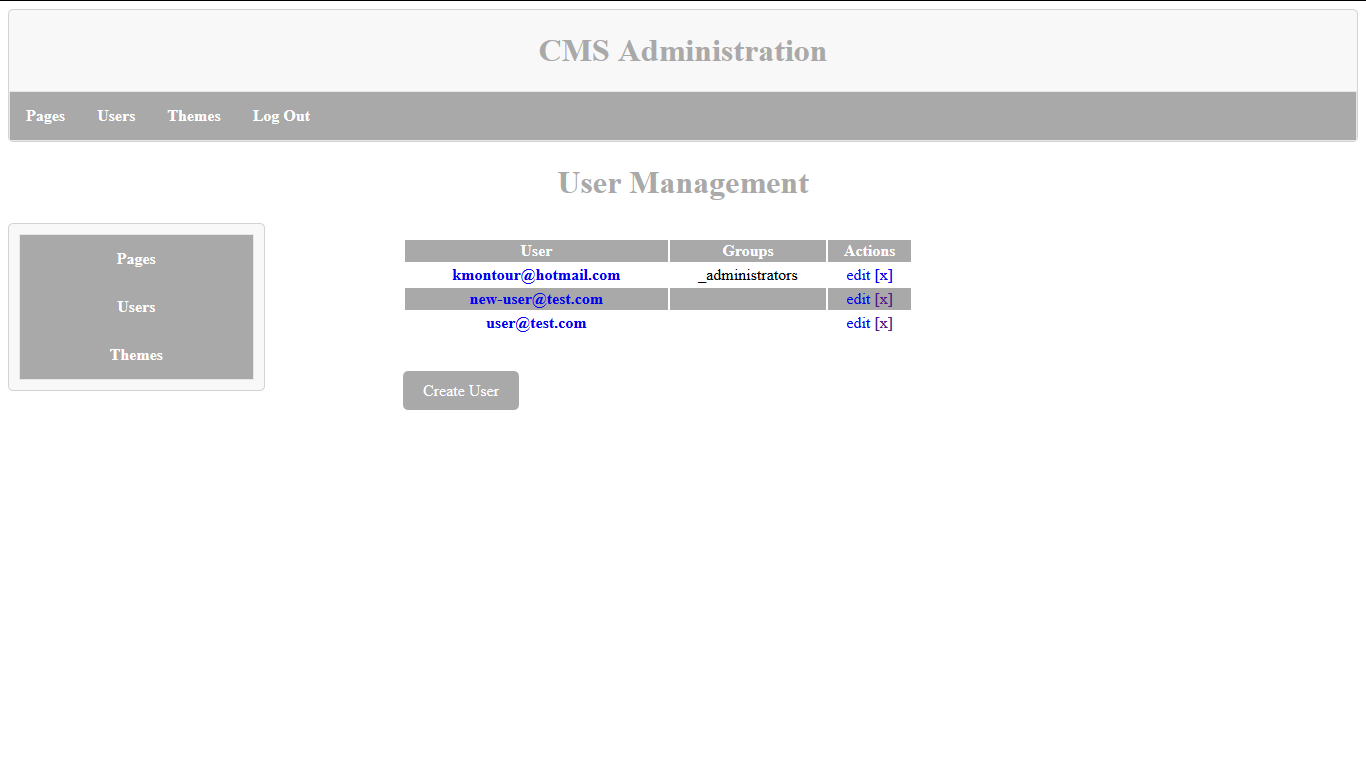
\includegraphics[width=\textwidth,height=\textheight,keepaspectratio]{pics/deleteUser_1.png}
  
  \item Click the [x] button pertaining to the user account that you would like to delete.
  
  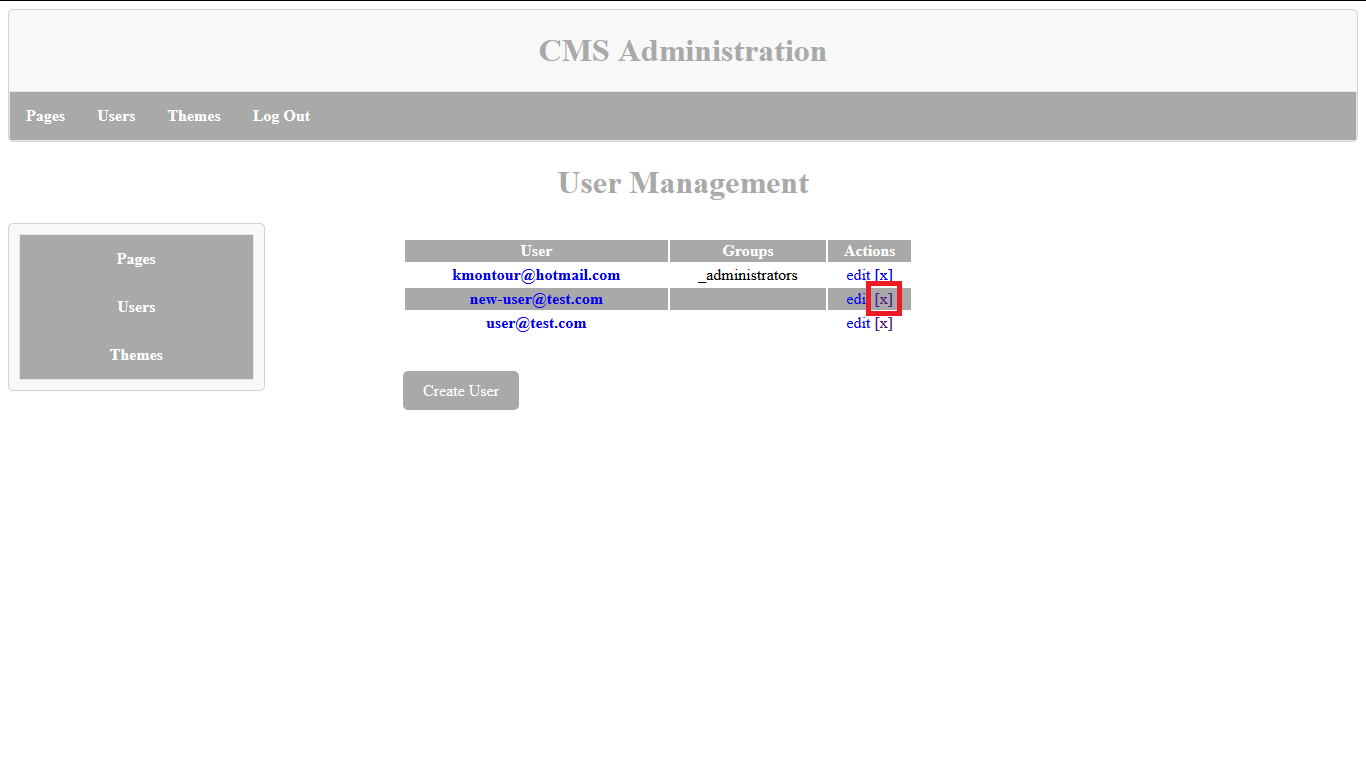
\includegraphics[width=\textwidth,height=\textheight,keepaspectratio]{pics/deleteUser_2.png}
  
  \item This brings up a Delete confirmation dialog box. Click ok to confirm the user account deletion.
  
  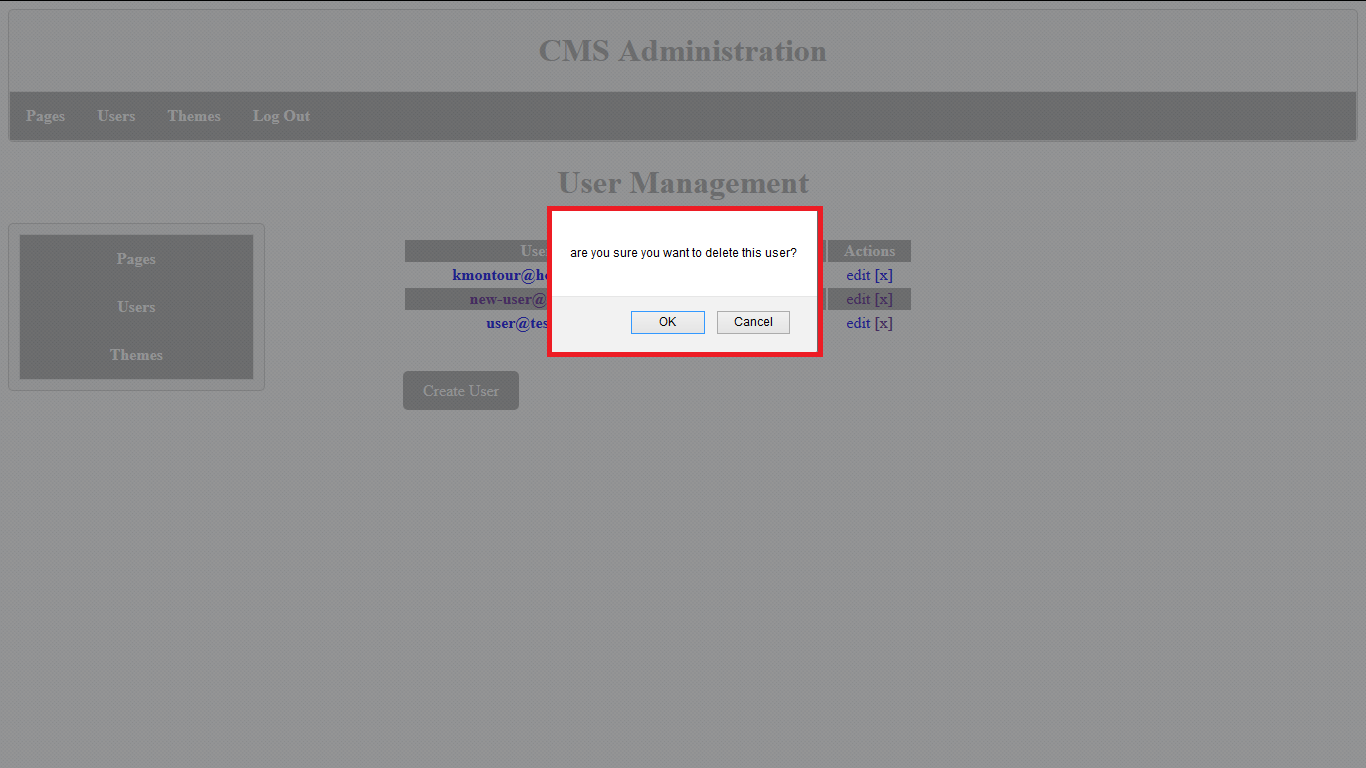
\includegraphics[width=\textwidth,height=\textheight,keepaspectratio]{pics/deleteUser_3.png}
  
  \item A list of user accounts is displayed with the deleted user account not in the list.
  
  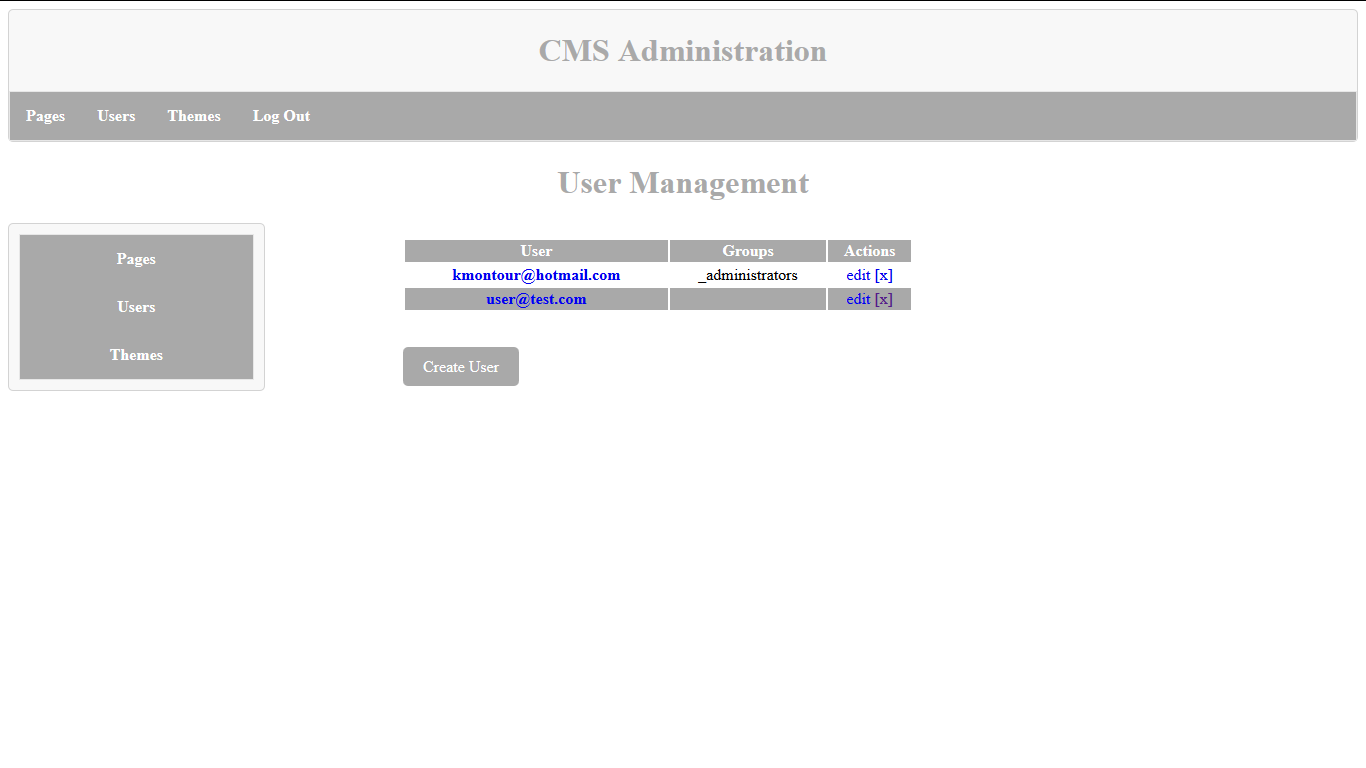
\includegraphics[width=\textwidth,height=\textheight,keepaspectratio]{pics/deleteUser_4.png}
  
  
\end{enumerate}

\subsection{Add a page through Page editor}

\begin{enumerate}
  \item Login to the administration web site (see above Login instructions). This brings you by default to the Page Management system.
  
  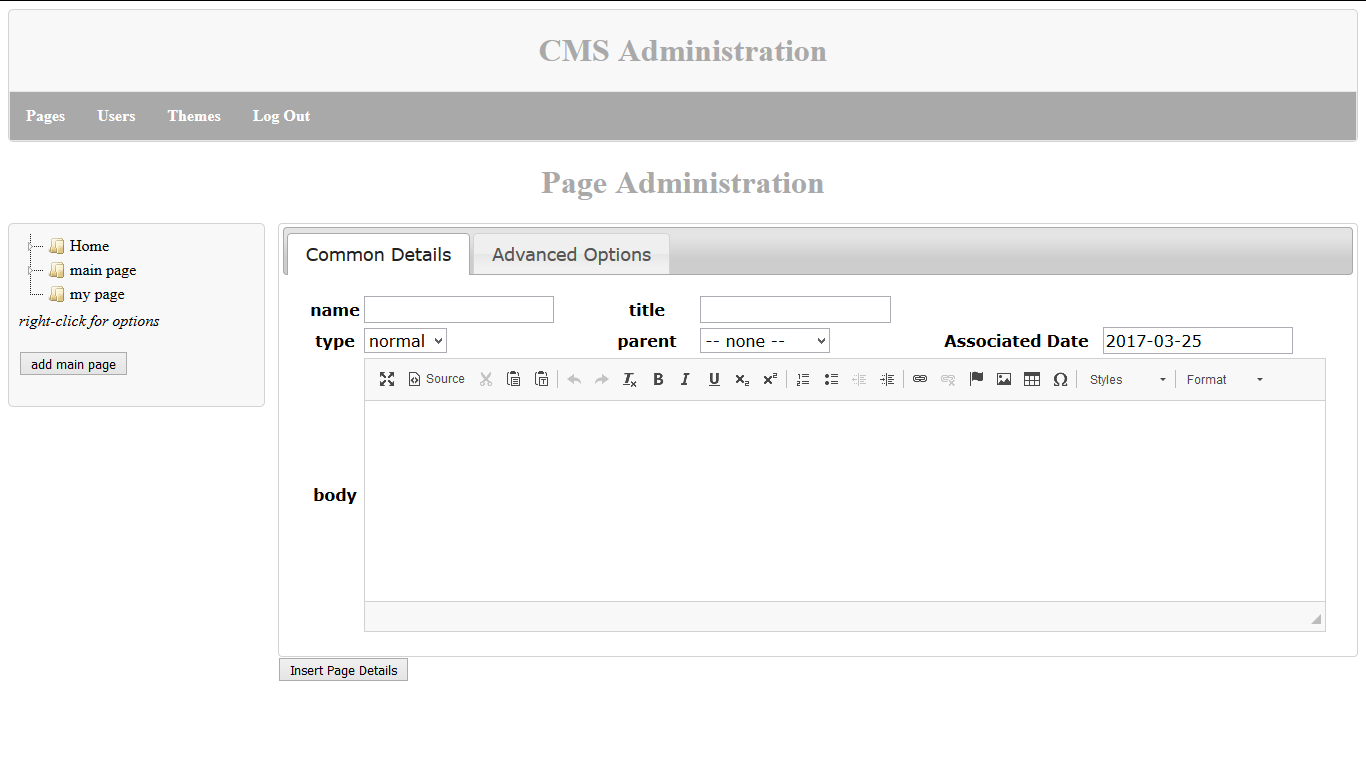
\includegraphics[width=\textwidth,height=\textheight,keepaspectratio]{pics/addPageThroughEditor_1.png}
  
  \item To create a new page, enter a page name into the name text box; enter a title for the page into the title text box; select a parent for the page, for this example ''none'' will be selected; enter a date into the Associated Date text box; enter web page content into the body text area. Finally, click the “Insert Page Details” to create the new page.
  
  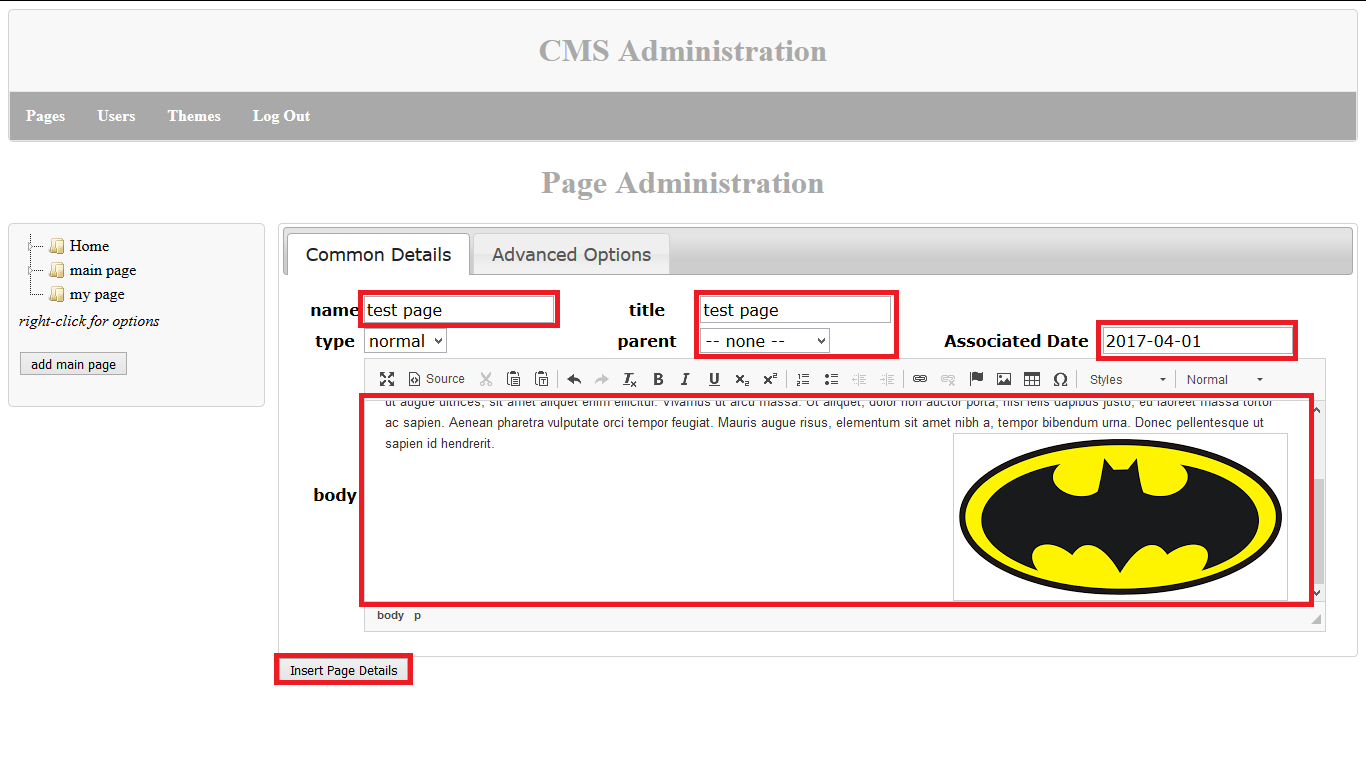
\includegraphics[width=\textwidth,height=\textheight,keepaspectratio]{pics/addPageThroughEditor_2.png}
  
  \item The page now shows up in the right page menu tree, with the page editor loaded with the inserted page data, and with a ''page saved'' message.
  
  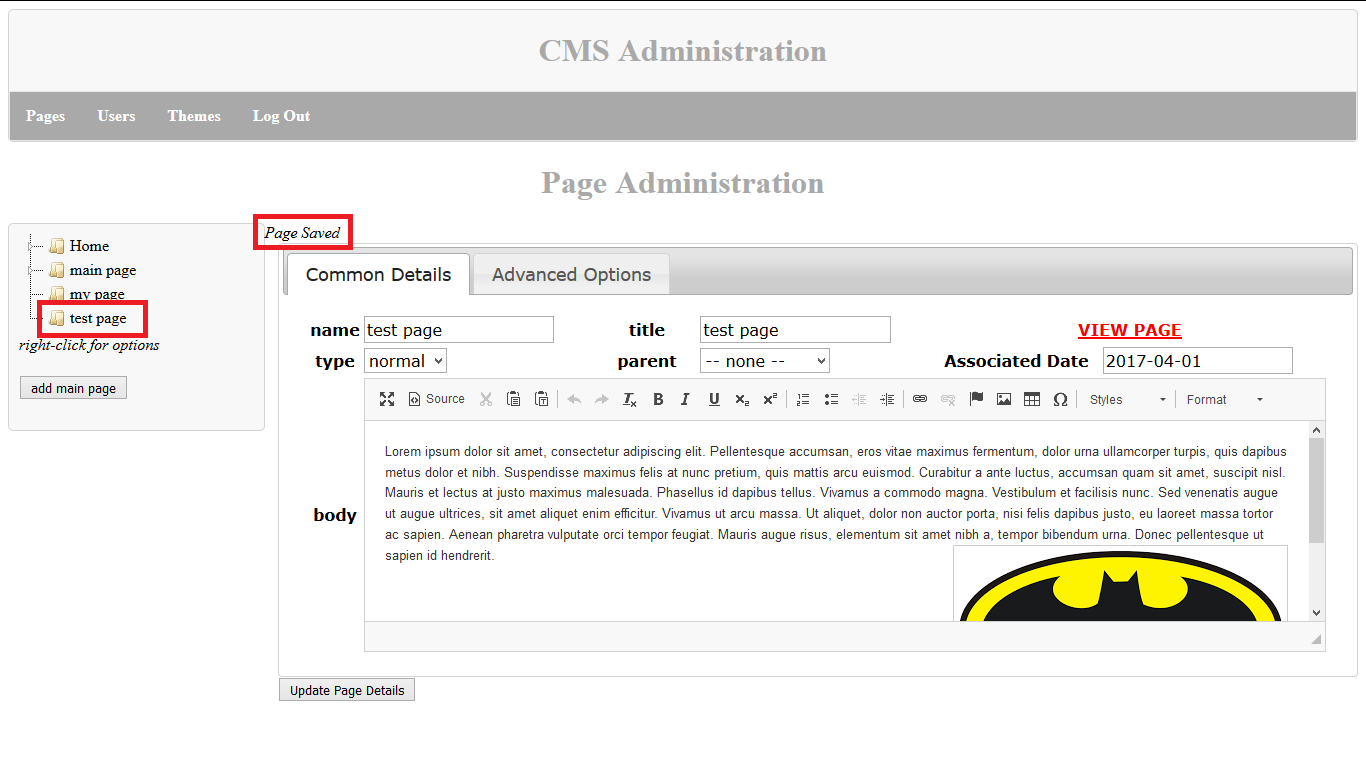
\includegraphics[width=\textwidth,height=\textheight,keepaspectratio]{pics/addPageThroughEditor_3.png}
  
  \item To view the newly inserted page on the front end, click the ''VIEW PAGE'' link.
  
  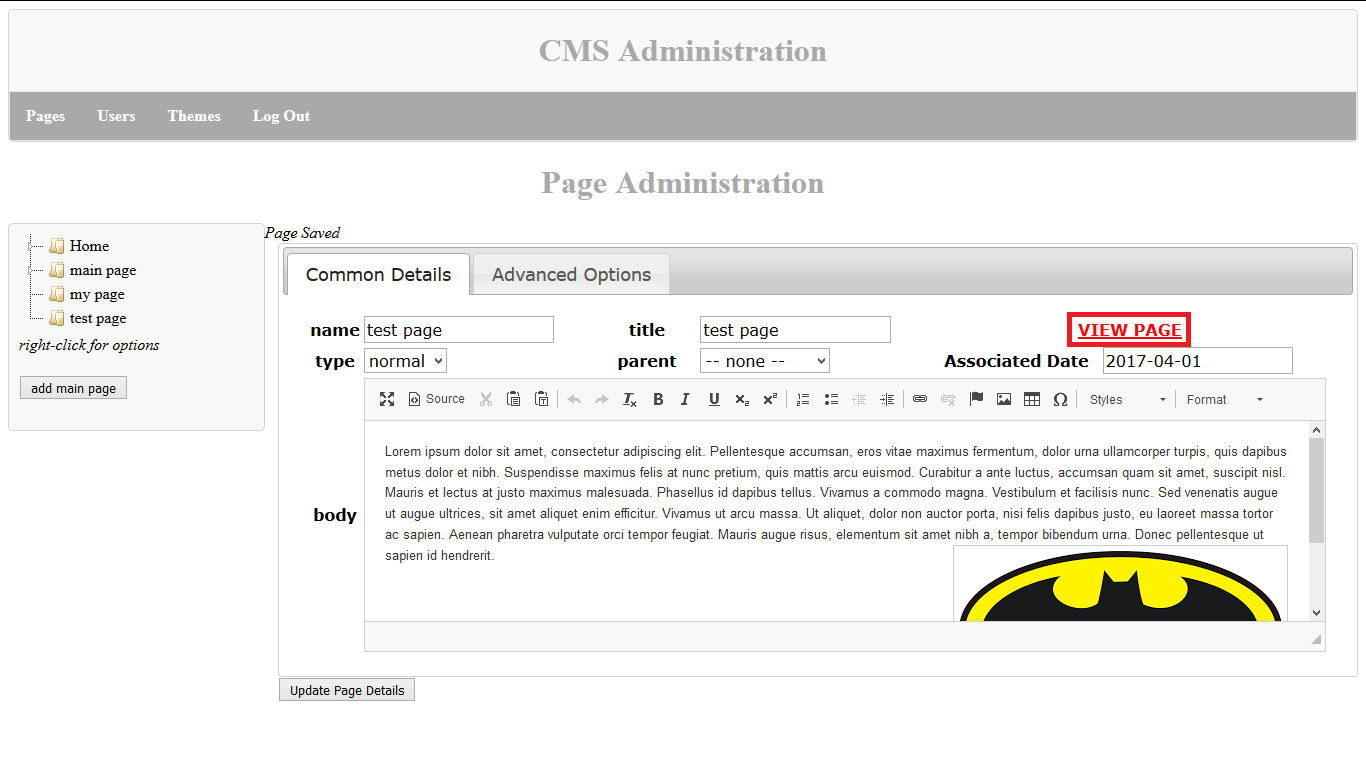
\includegraphics[width=\textwidth,height=\textheight,keepaspectratio]{pics/addPageThroughEditor_4.png}
  
  \item Clicking the ''VIEW PAGE'' button opens a new tab with the newly created page content displayed in the currently selected template.
  
  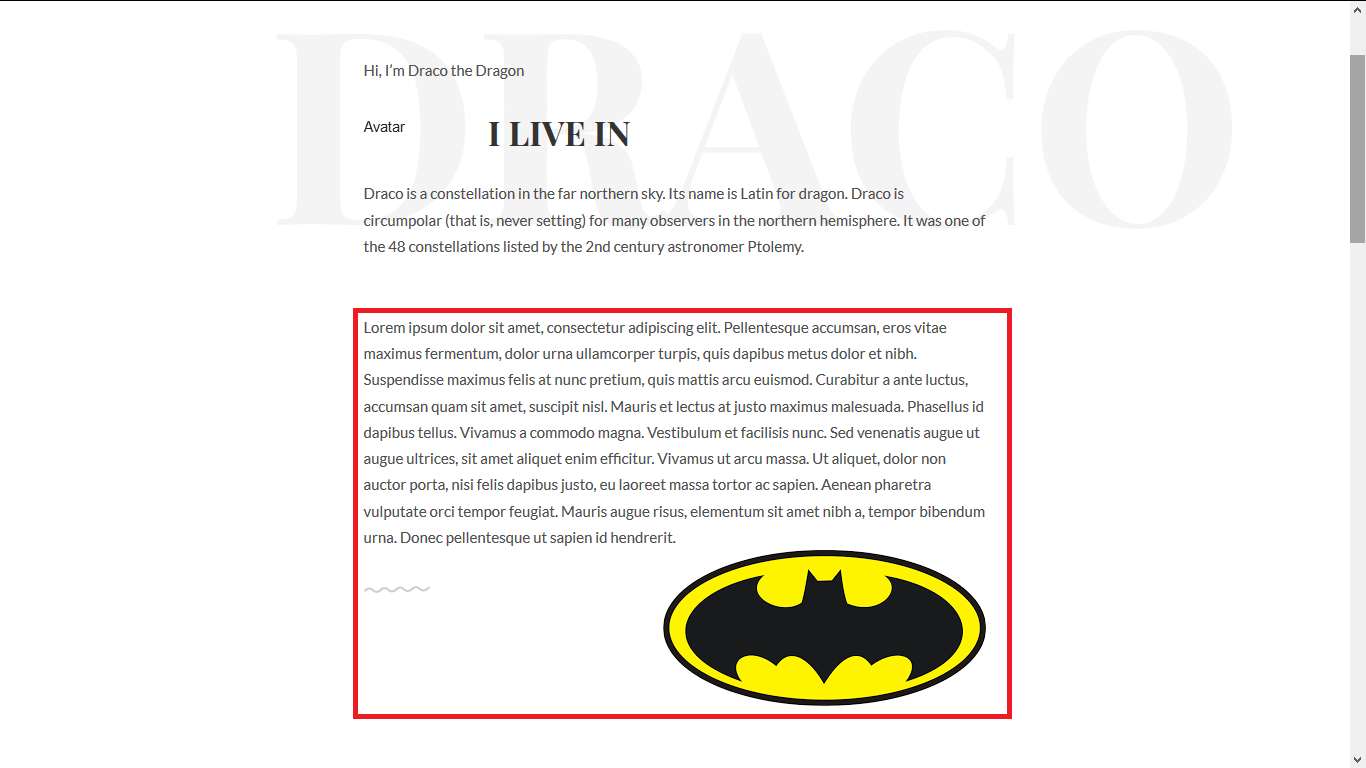
\includegraphics[width=\textwidth,height=\textheight,keepaspectratio]{pics/addPageThroughEditor_5.png}
  
  
\end{enumerate}

\subsection{Add main page through page tree ''add main page'' button}

\begin{enumerate}
  \item Login to the administration web site (see above Login instructions). This brings you by default to the Page Management system.
  
  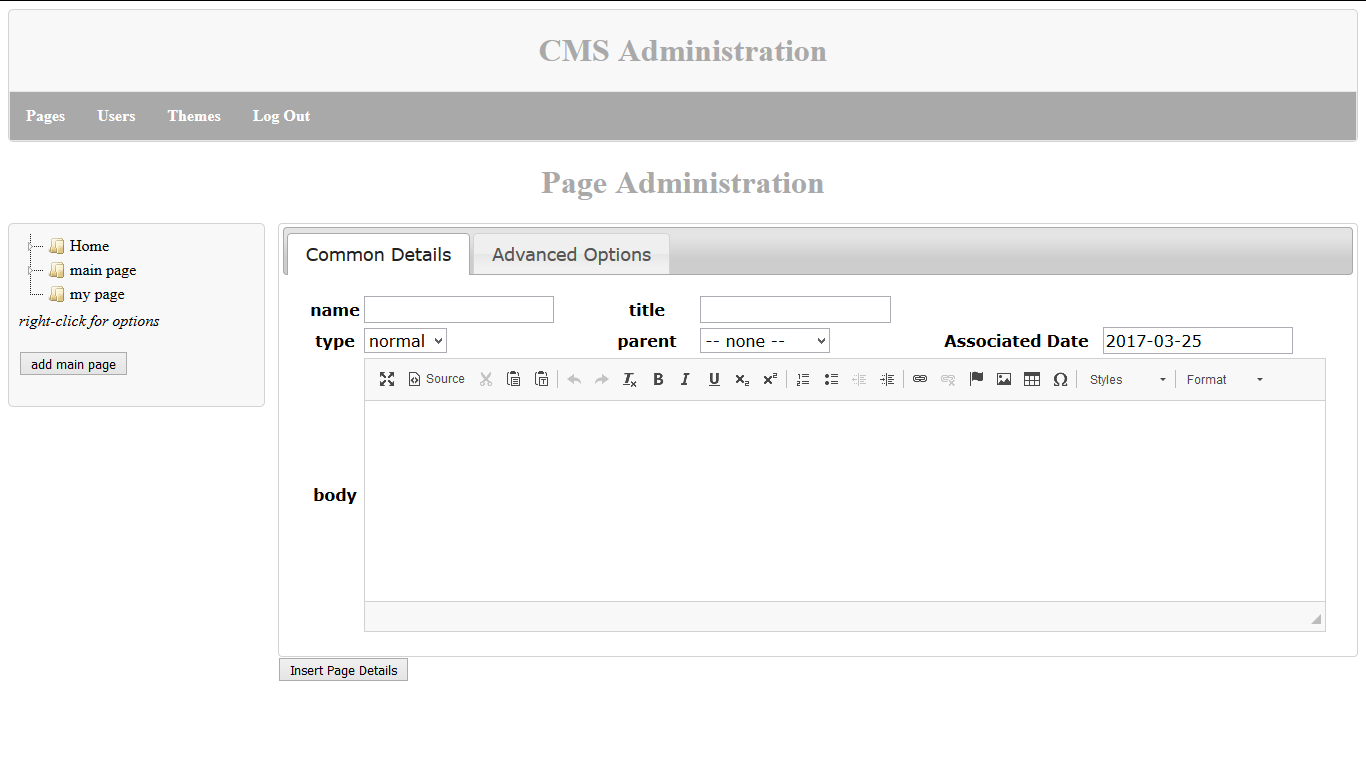
\includegraphics[width=\textwidth,height=\textheight,keepaspectratio]{pics/mainPageButton_1.png}
  
  \item To create a top level page with the ''add main page'' button, click the ''add main page'' button in the page tree menu on the left.
  
  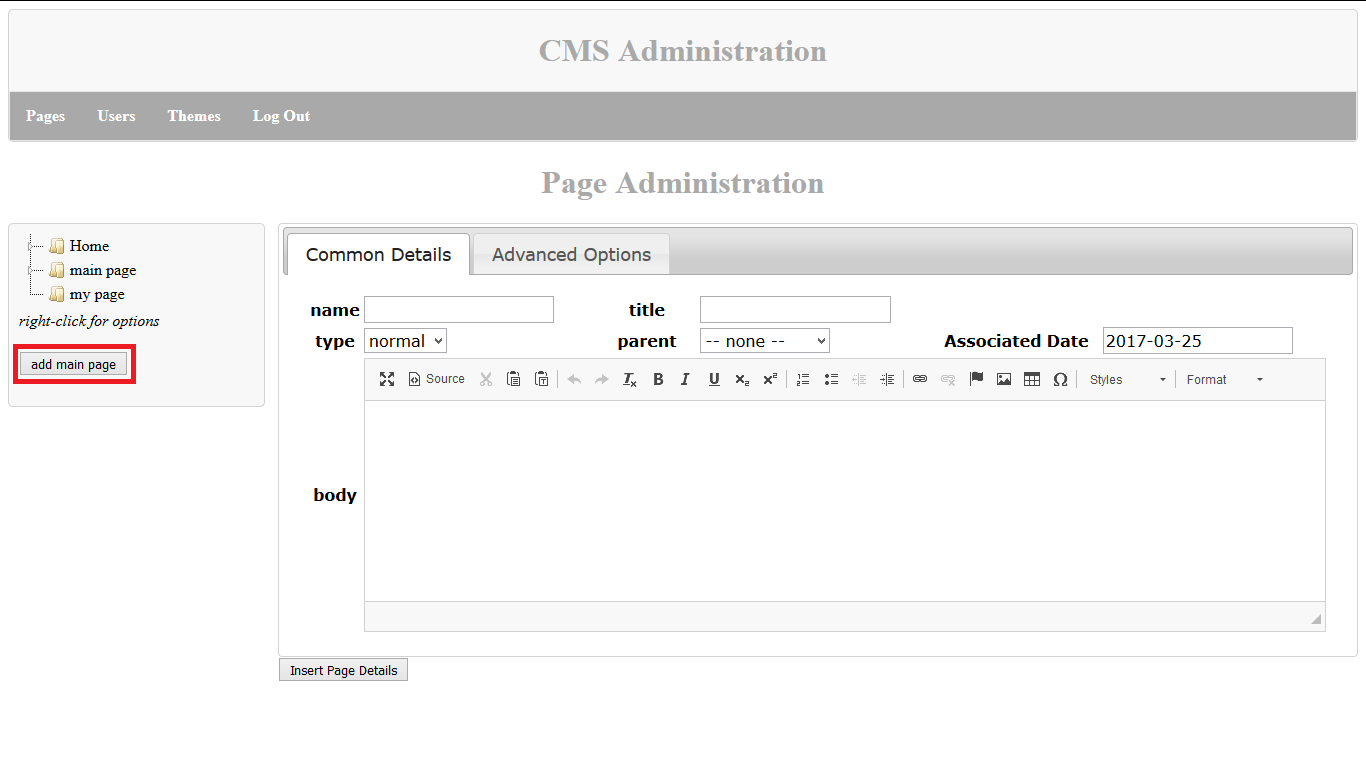
\includegraphics[width=\textwidth,height=\textheight,keepaspectratio]{pics/mainPageButton_2.png}
  
  \item Clicking the ''add main page'' button brings up a page creation dialog box. Enter a page name in the Name input text box; Select a page type from the Page Type drop down list; Select a date from the date picker for the Associated input box. Then click the ''Create Page'' button to create the page.
  
  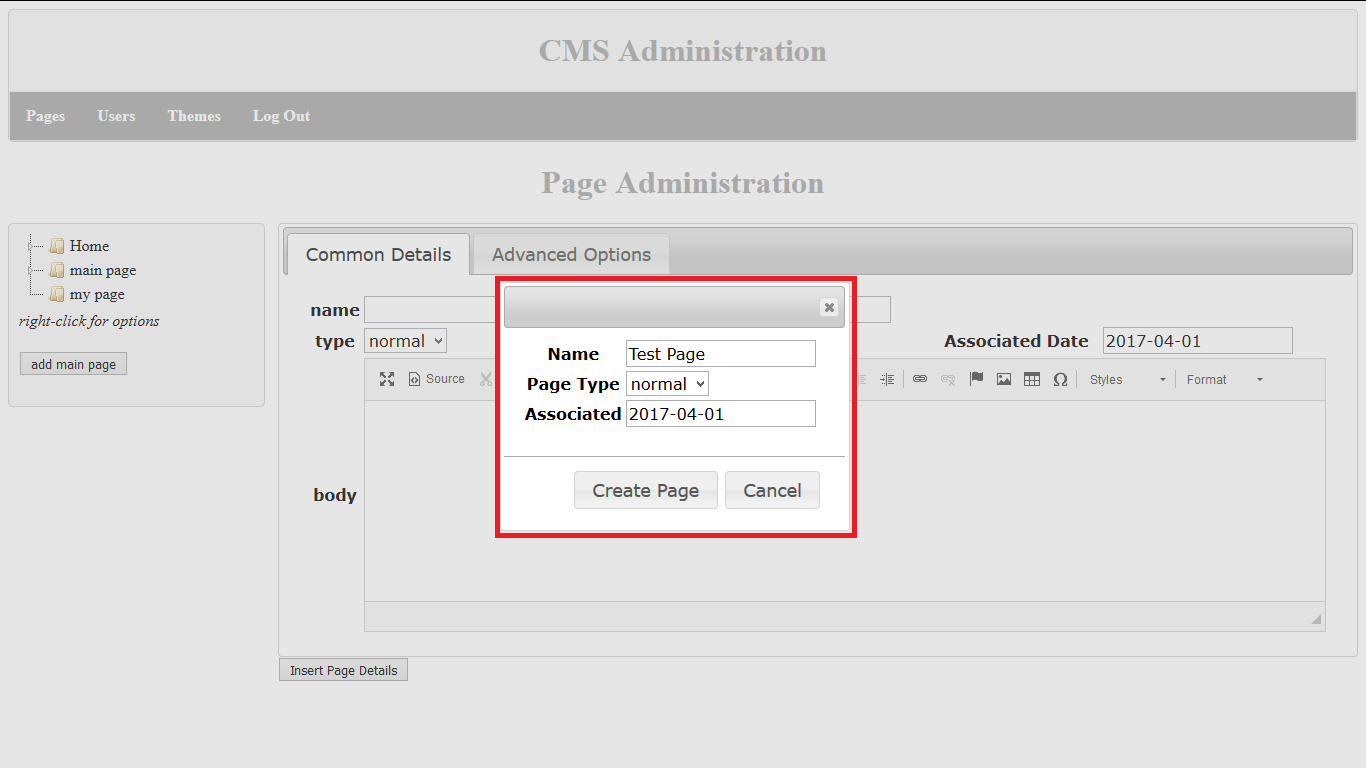
\includegraphics[width=\textwidth,height=\textheight,keepaspectratio]{pics/mainPageButton_3.png}
  
  \item Clicking the ''Create Page'' button creates the unfinished page, displays a ''Page Saved'' message, displays the unfinished newly created page in the page tree menu on the left, and loads the newly created page data into the page editor.
  
  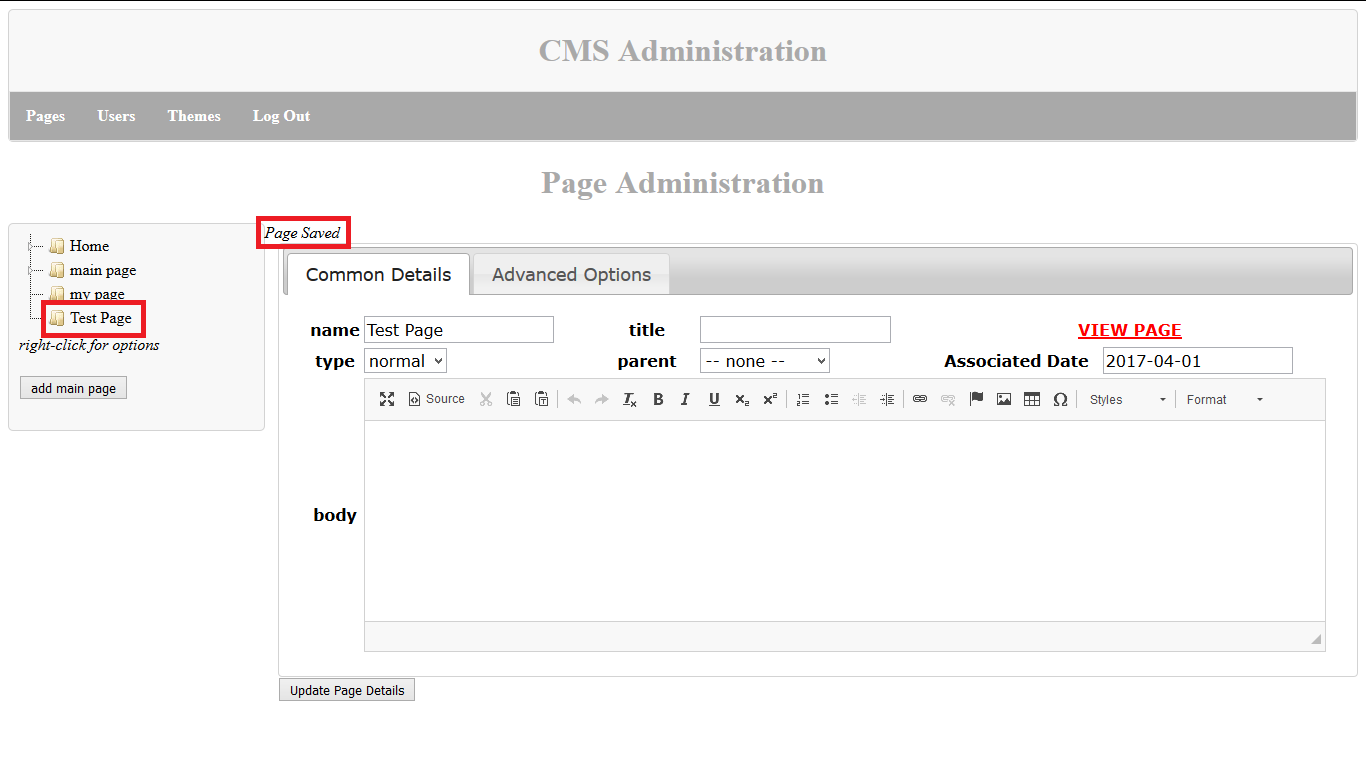
\includegraphics[width=\textwidth,height=\textheight,keepaspectratio]{pics/mainPageButton_4.png}
  
  \item To see the incomplete ''Test Page'' completed, see the instructions for editing a page.
  
\end{enumerate}


\subsection{Edit Page}

\begin{enumerate}
  \item Login to the administration web site (see above Login instructions). This brings you by default to the Page Management system.
  
  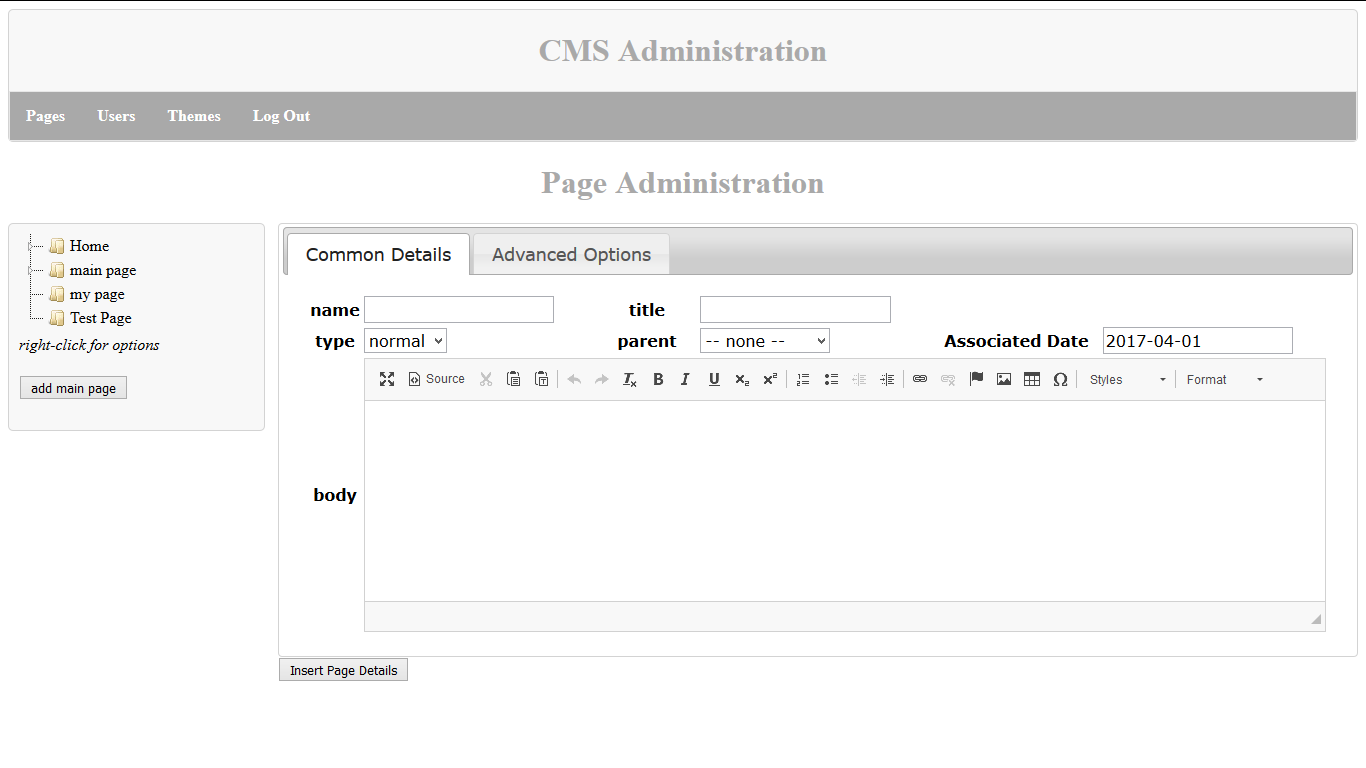
\includegraphics[width=\textwidth,height=\textheight,keepaspectratio]{pics/editPage_1.png}
  
  \item Click the ''Test Page'' link in the page tree menu on the left.
  
  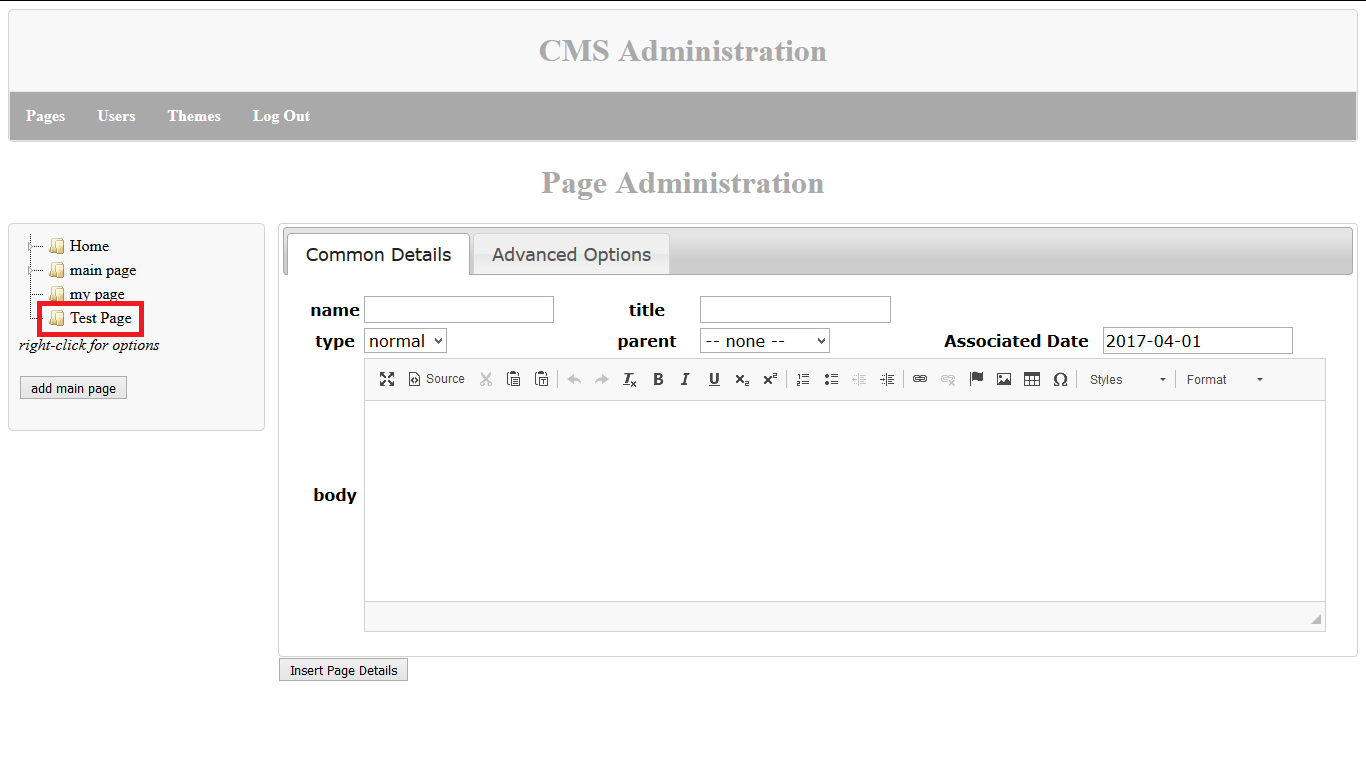
\includegraphics[width=\textwidth,height=\textheight,keepaspectratio]{pics/editPage_2.png}
  
  \item Clicking the ''Test Page'' link loads the page editor with the ''Test Page'' data ready for editing.
  
  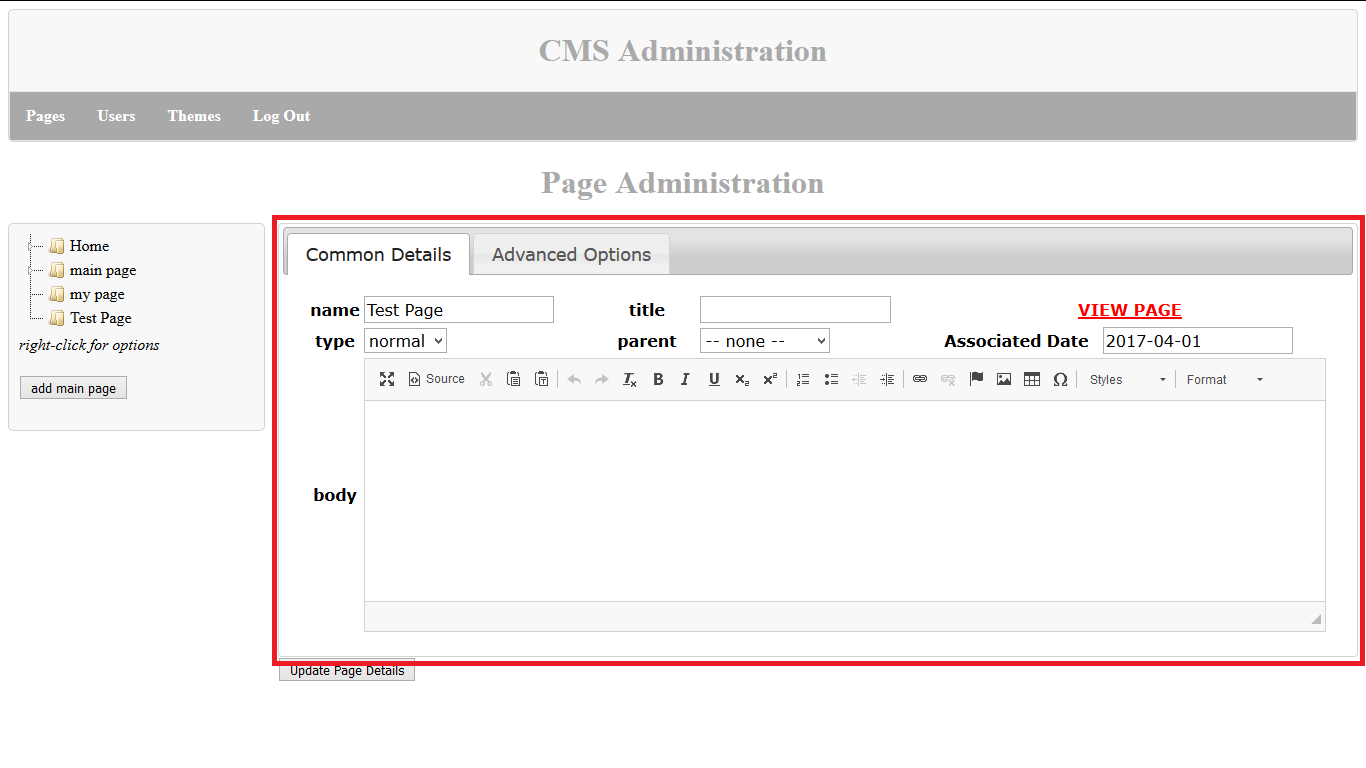
\includegraphics[width=\textwidth,height=\textheight,keepaspectratio]{pics/editPage_3.png}
  
  \item Edit the ''Test Page'' by entering a page title into the title input box and entering some web page content into the body text area, and click the ''Update Page Details'' button. 
  
  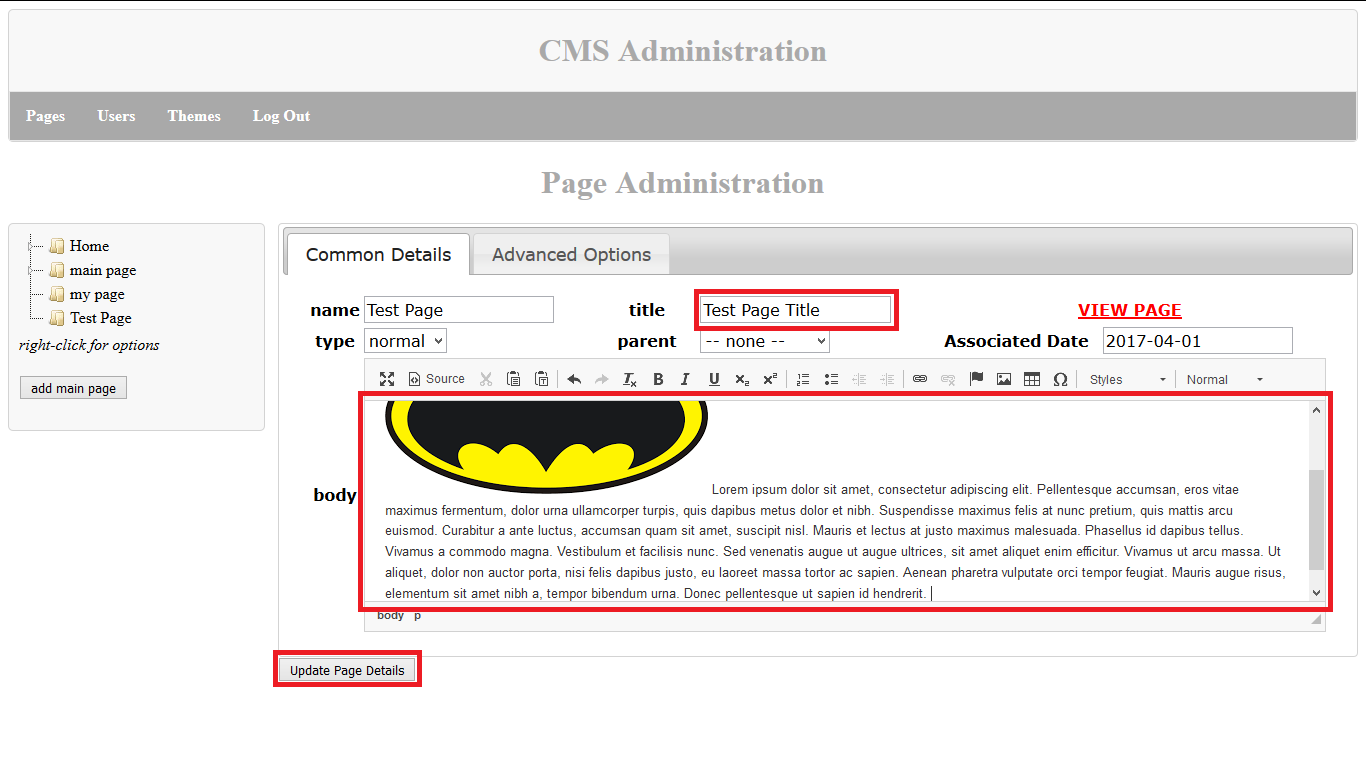
\includegraphics[width=\textwidth,height=\textheight,keepaspectratio]{pics/editPage_4.png}
  
  \item Clicking the ''Update Page Details'' updates the “Test Page” with the new data, displays a ''Page Saved'' message, and reloads the page editor with the updated page data.
  
  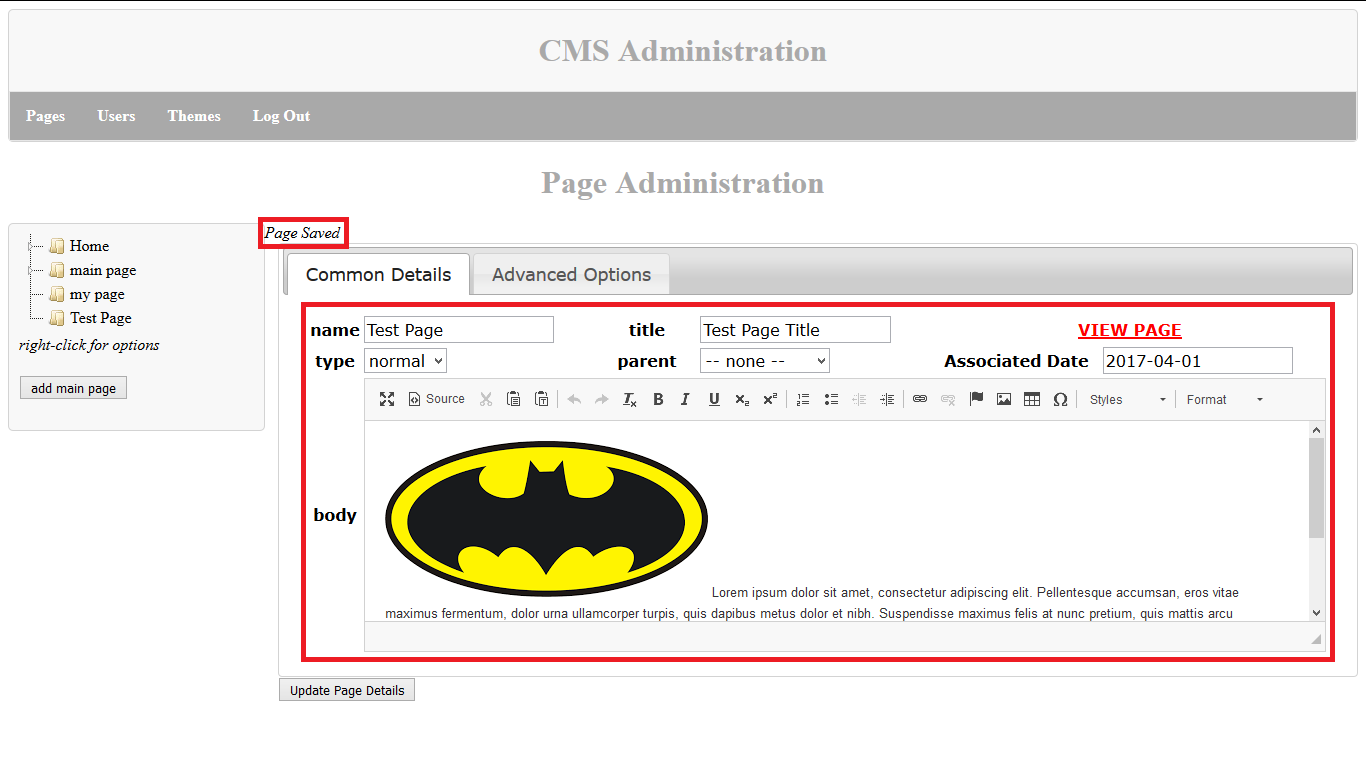
\includegraphics[width=\textwidth,height=\textheight,keepaspectratio]{pics/editPage_5.png}
  
  \item To view the updated page on the front-end, click the ''VIEW PAGE'' button.
  
  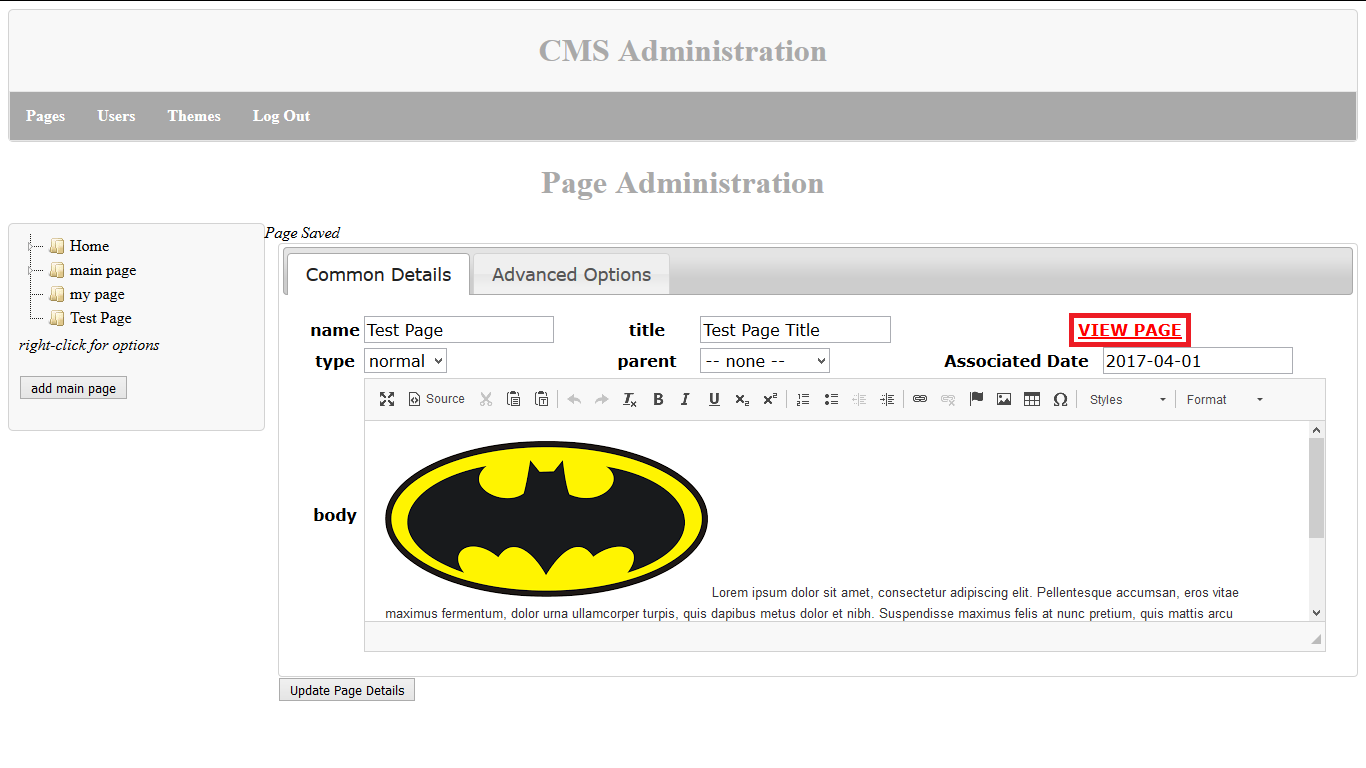
\includegraphics[width=\textwidth,height=\textheight,keepaspectratio]{pics/editPage_6.png}
  
  \item Clicking the ''VIEW PAGE'' button opens a new tab, loads the updated page content into the current template and displays the updated page in the browser.
  
  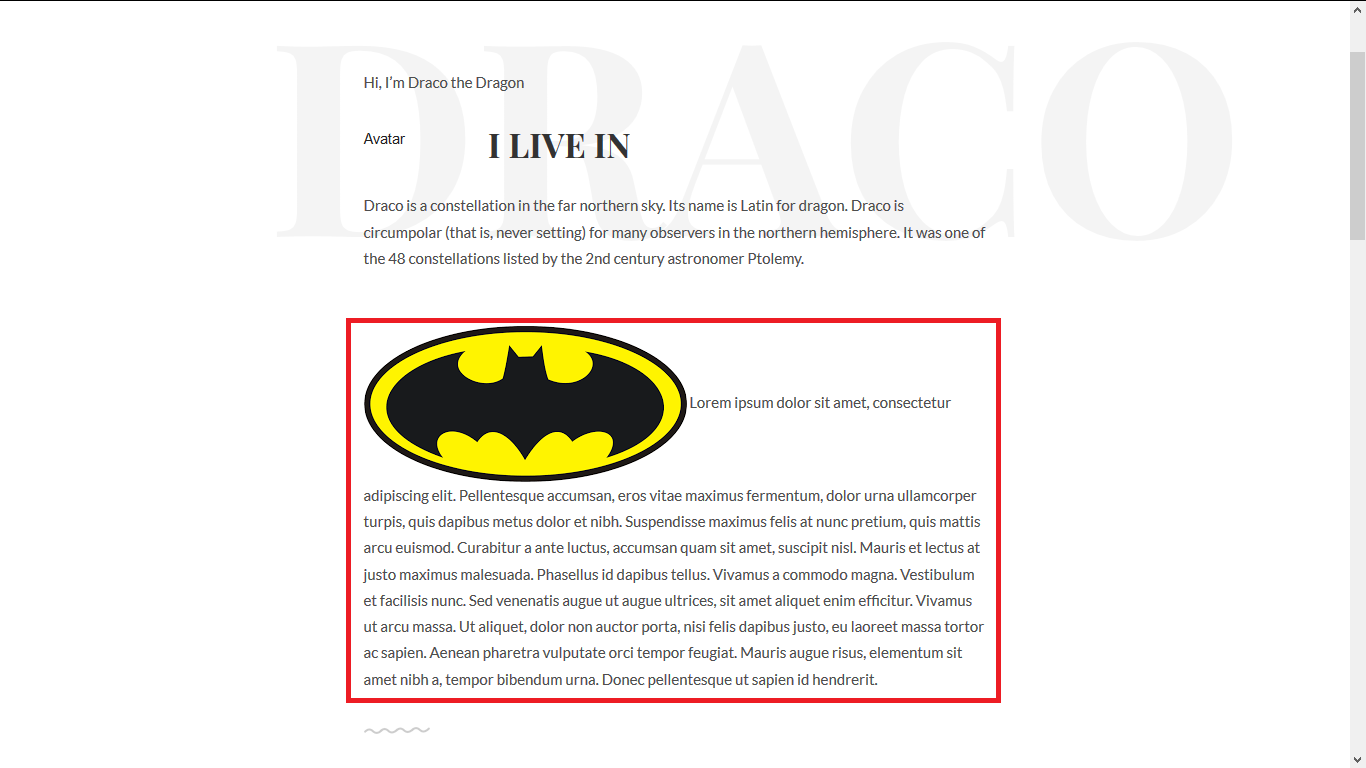
\includegraphics[width=\textwidth,height=\textheight,keepaspectratio]{pics/editPage_7.png}
    
\end{enumerate}

\subsection{Add child page with context menu}
\begin{enumerate}
  \item Login to the administration web site (see above Login instructions). This brings you by default to the Page Management system.
  
  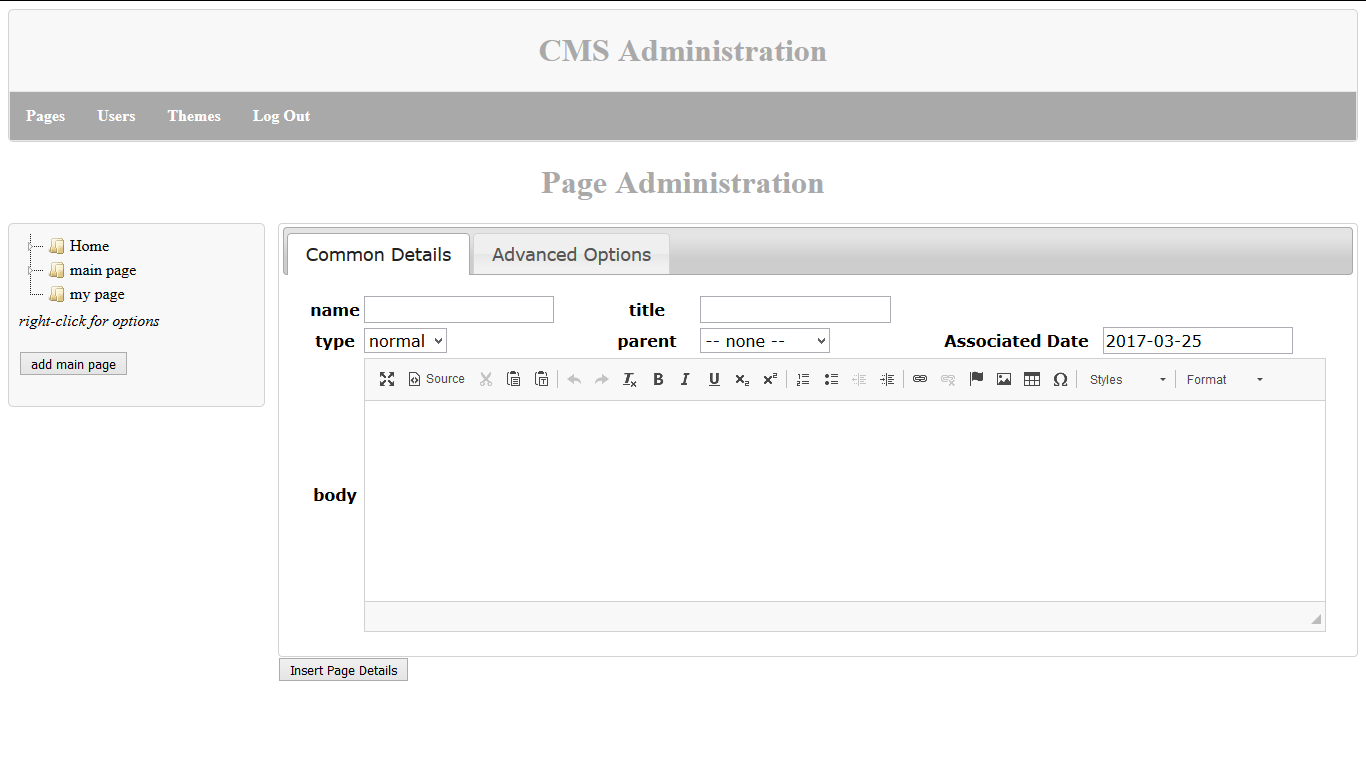
\includegraphics[width=\textwidth,height=\textheight,keepaspectratio]{pics/childPageWithContextMenu_1.png}
  
  \item To create a child page, right click the page you have selected to be the parent and, select the ''Create Page'' menu option.
  
  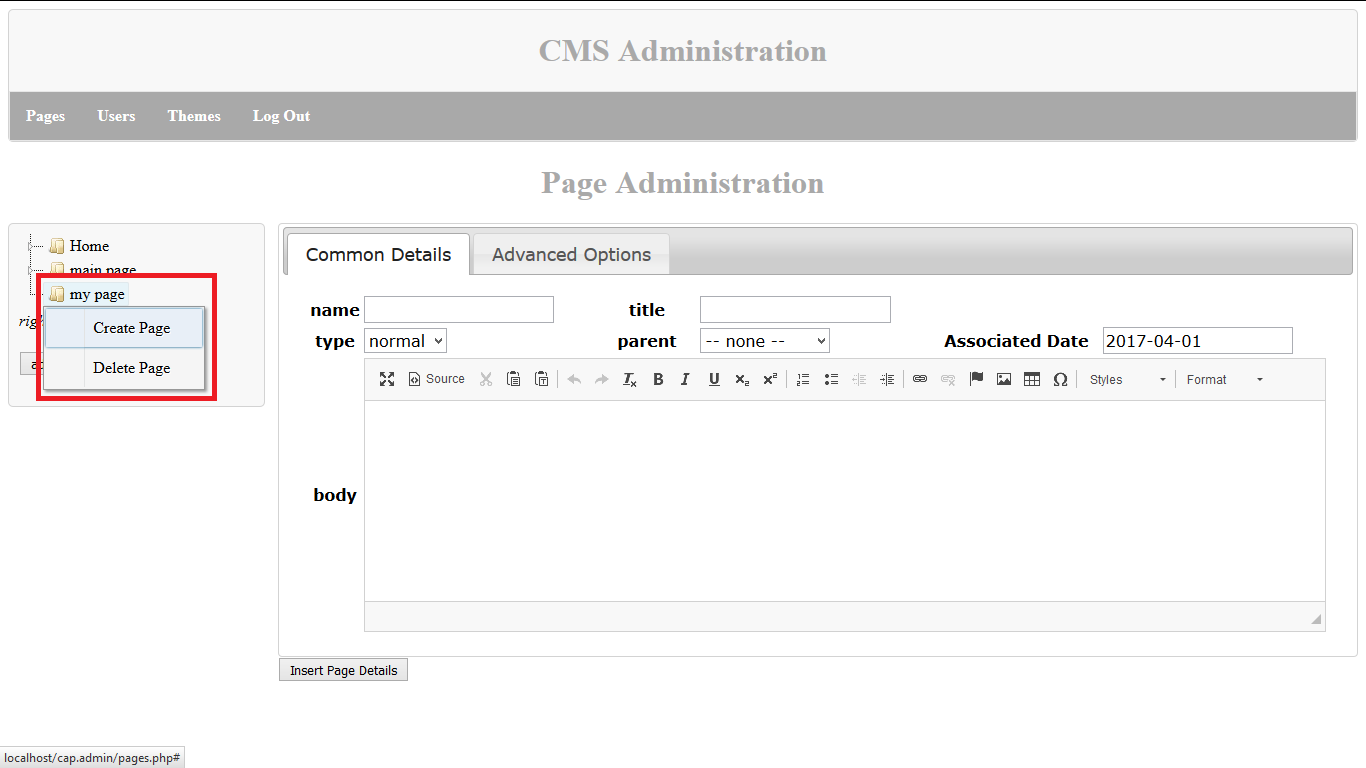
\includegraphics[width=\textwidth,height=\textheight,keepaspectratio]{pics/childPageWithContextMenu_2.png}
  
  \item Selecting ''Create Page'' from the context menu of a parent page brings up a Create Page dialog for creating a new child page. Enter a page name in the Name input text box; Select a page type from the Page Type drop down list; Select a date from the date picker for the Associated input box. Then click the ''Create Page'' button to create the page.
  
  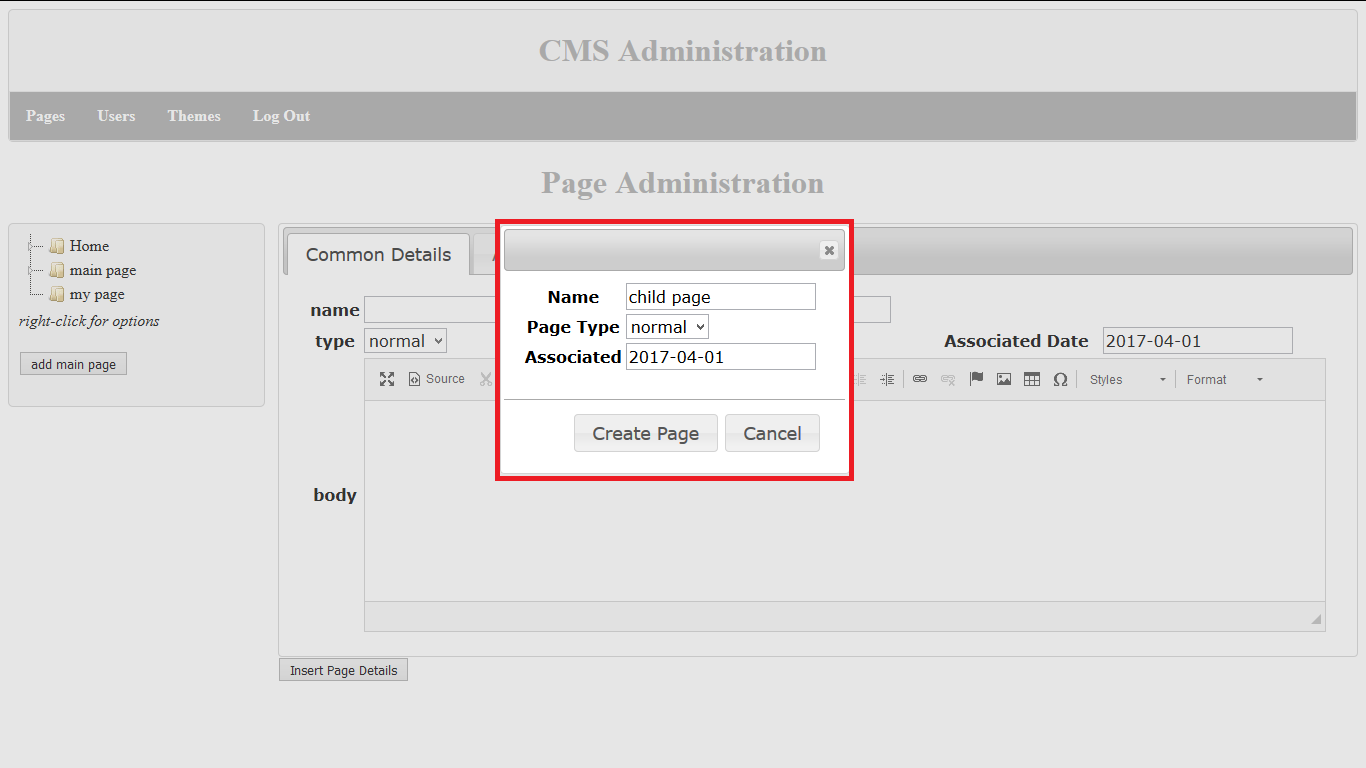
\includegraphics[width=\textwidth,height=\textheight,keepaspectratio]{pics/childPageWithContextMenu_3.png}
  
  \item Clicking the ''Create Page'' button creates the unfinished child page, displays a ''Page Saved'' message, displays the unfinished newly created child page in the page tree menu on the left under the selected parent page, and loads the newly created page data into the page editor.
  
  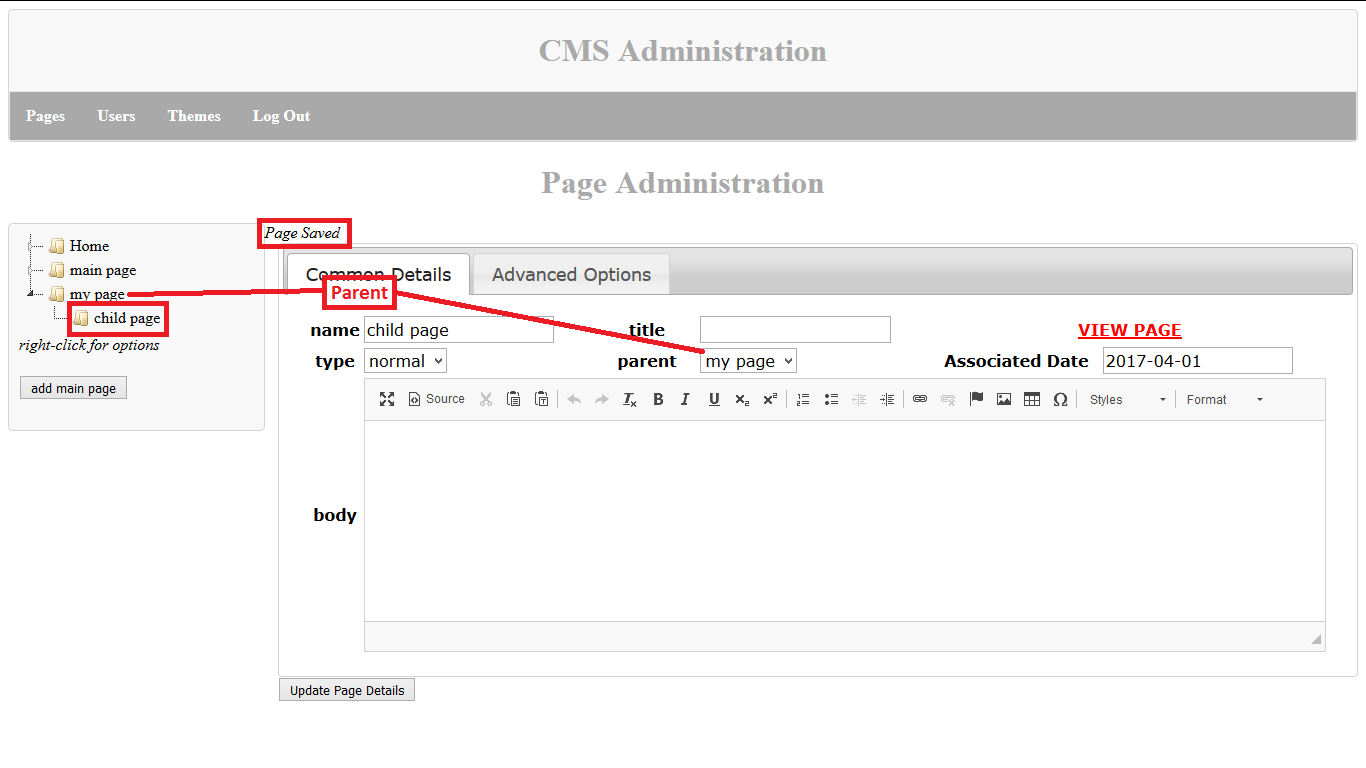
\includegraphics[width=\textwidth,height=\textheight,keepaspectratio]{pics/childPageWithContextMenu_4.png}
  
  
  \item To finish the partially completed child page see above instructions on editing pages.
  

\end{enumerate}





\end{document}